\chapter{Linear Algebra}
\label{ch:linear}

\section{Row Operations and Echelon Form}

\begin{defn}\label{linear-eq}
    A \emph{linear equation} is an equation of the form $a_1x_1 + a_2x_2 + \cdots + a_nx_n = b$
\end{defn}

\begin{defn}\label{linear-sys}
    A \emph{system of linear equations} (or \emph{linear system}) is a set of linear equations of the same variables (e.g. $x_1, x_2, \ldots, x_n$).
\end{defn}

\begin{defn}\label{linear-sys-solutions}
    The \emph{solution set} of a system of linear equations is the intersection of the solution set of each individual linear equation.
\end{defn}

Systems of linear equations can be represented via matrices, where each column is a specific variable, each row is a linear equation, and the entries are the coefficients. Augmentations represent the constant term (denoted $b$ in definition \ref{linear-eq}).

\begin{exmp}
    The linear system \[\begin{linsys}{3}
            x &+ &2y &- &z &= &-1 \\
            2x &+ &2y &+ &z &= &1 \\
            3x &+ &5y &- &2z &= &-1
        \end{linsys}\] can be represented by the augmented matrix below.
    \[\begin{amatrix}{3}
            1 &2 &-1 &-1 \\
            2 &2 &1 &1 \\
            3 &5 &-2 &-1
        \end{amatrix}\]
\end{exmp}

Row operations are certain operations on matrices or systems of linear equations which can be used to simply or otherwise transform the system, while leaving the solution set unchanged.

\begin{defn}\label{row-op}
    Row operations: \begin{enumerate}
        \item Swap two rows/equations
        \item Multiply a single row by a non-zero scalar
        \item Add a scalar multiple of one row to another
    \end{enumerate}
\end{defn}

\begin{thm}\label{solutions-unchanged-by-row-ops}
    If a linear system is obtained from another by one of the row operations, then the two systems have the same set of solutions.
\end{thm}

\begin{proof}\proofbreak
    \begin{enumerate}
        \item As the intersection of sets is commutative, by Definition \ref{linear-sys-solutions}, the solution set of a linear system is unaffected by the order of the individual linear systems, therefore swapping rows/equations does not change the solution set.
        \item Since multiplying a single row by a non-zero scalar is equivalent to multiplying both sides of the represented equation by that scalar, the solution set is clearly left unchanged.
        \item Since adding a multiple of one row to another row is equivalent to adding equal quantities to both sides of the equation, no solutions are removed from the solution set. If the row $(sb_1 + a_1)x_1 + (sb_2 + a_2) + \cdots + (sb_n + a_n)x_n = sk_b + k_a$ is the result of adding $s$ times row $b_1x_1 + \cdots + b_nx_n = k_b$ to row $a_1x_1 + \cdots + a_nx_n = k_a$, then $(sb_1 + a_1)x_1 + (sb_2 + a_2) + \cdots + (sb_n + a_n)x_n = s(b_1x_1 + \cdots + b_nx_n) + k_a$  which implies that $a_1x_1 + \cdots + a_nx_n = k_a$, so no information was lost, and the solution set remains the same.
    \end{enumerate}
\end{proof}

\begin{defn}
    A matrix in (row) \emph{echelon form} has all rows of zeroes at the bottom, and the leading term of each row is to the right of the row leading term above it.
\end{defn}

\begin{defn}
    In \emph{reduced row echelon form}, a matrix in row echelon form additionally has leading terms which are all $1$, and the entries above and below each leading term are zero.
\end{defn}

\begin{rmk}
    The reduced row echelon form of a particular matrix is always unique, however the row echelon form is not. Additionally, it is always possible to transform a given matrix into either echelon form via the row operations.
\end{rmk}

\begin{exmp}
    \begin{align*}
        \begin{amatrix}{3}
            1 &0 &1 &4 \\
            1 &-1 &2 &5 \\
            4 &-1 &5 &17
        \end{amatrix}
         & \begin{aligned}
             & \ro{r_2 \rightarrow r_2 - r_1}  \\
             & \ro{r_3 \rightarrow r_3 - 4r_1} \\
        \end{aligned}
         & \begin{amatrix}{3}
            1 &0 &1 &4 \\
            0 &-1 &1 &1 \\
            0 &-1 &1 &1
        \end{amatrix}
         & \begin{aligned}
             & \ro{r_2 \rightarrow -r_2} \\
        \end{aligned}
         & \begin{amatrix}{3}
            1 &0 &1 &4 \\
            0 &1 &-1 &-1 \\
            0 &-1 &1 &1
        \end{amatrix} \\
         & \begin{aligned}
             & \ro{r_3 \rightarrow r_3 + r_2} \\
        \end{aligned}
         & \begin{amatrix}{3}
            1 &0 &1 &4 \\
            0 &1 &-1 &-1 \\
            0 &0 &0 &0
        \end{amatrix}
    \end{align*}

    Since there is no leading term corresponding to $z$, $z$ is a free variable. If we let $z$ be zero, then the augmentation yields a particular solution to this linear system.

    Solution set in vector form:
    \[\begin{pmatrix}
            x \\ y \\ z
        \end{pmatrix} = \begin{pmatrix}
            4 \\ -1 \\ 0
        \end{pmatrix} + z\begin{pmatrix}
            -1 \\ 1 \\ 1
        \end{pmatrix}\]

    Solution set in parametric form:
    \[\left\{\left(4 - z, -1 + z, z\right) \compbar z \in \R \right\}\]

\end{exmp}

\section{Vector Spaces}

\begin{defn}
    Let $F$ be a field. A \emph{vector space} over $F$ consists of a set $V$ together with two operations:

    \begin{itemize}
        \item[] $+: V \times V \to V$ (vector addition)
        \item[] $\cdot: F \times V \to V$ (scalar multiplication)
    \end{itemize}
    which satisfy the following axioms for all $v, w, e \in V$ and $r, s \in F$:
    \begin{enumerate}
        \item $v + w = w + v$ (additive commutativity)
        \item $(v + w) + u = v + (w + u)$ (additive associativity)
        \item $\exists \vec{0} \in V \textrm{ s.t. } v + \vec{0} = v$ (additive identity)
        \item $\exists z \in V \textrm{ s.t. } v + z = \vec{0}$ (additive inverse)
        \item $(r + s) \cdot v = r \cdot v + s \cdot v$ (distributivity over scalar addition)
        \item $r \cdot (v + w) = r \cdot v + r \cdot w$ (distributivity over vector addition)
        \item $(rs)\cdot v = r \cdot (s \cdot v)$ (multiplicative associativity)
        \item $1 \cdot v = v$ (multiplicative identity)
    \end{enumerate}
\end{defn}

\begin{rmk}
    You can prove the following for all $v \in V$ and $r \in F$ from those axioms (see Lemma \ref{vector-space-properties}):
    \begin{itemize}
        \item The additive identity ($\vec{0}$) is unique.
        \item Additive inverses are unique.
        \item $0 \cdot v = \vec{0}$.
        \item $-1 \cdot v = -v$.
        \item $r \cdot \vec{0} = \vec{0}$.
    \end{itemize}
\end{rmk}

\begin{exmp}
    $\R^n$ is a vector space over $\R$ with $+$ and $\cdot$ defined as usual.
\end{exmp}

\begin{exmp}
    Let $F$ be any field. Then \[F^n = \left\{\begin{pmatrix}
            x_1 \\ \vdots \\ x_n
        \end{pmatrix} \compbar x_i \in F \textrm{ for } i = 1, \ldots, n \right\}\] is a vector space over $F$ with $x + y$ defined as \[\begin{pmatrix}
            x_1 \\ \vdots \\ x_n
        \end{pmatrix} + \begin{pmatrix}
            y_1 \\ \vdots \\ y_n
        \end{pmatrix} = \begin{pmatrix}
            x_1 + y_1 \\ \vdots \\ x_n + y_n
        \end{pmatrix}\] and $r \cdot x$ defined as \[r\begin{pmatrix}
            x_1 \\ \vdots \\ x_n
        \end{pmatrix} = \begin{pmatrix}
            rx_1 \\ \vdots \\ rx_n
        \end{pmatrix}.\]
\end{exmp}

Consider the field $\mathbb{F}_2 = \{0, 1\}$, and the vector space $\mathbb{F}_2^2$. This vector space has four elements: $\left\{\begin{pmatrix}
        0 \\ 0
    \end{pmatrix}, \begin{pmatrix}
        0 \\ 1
    \end{pmatrix}, \begin{pmatrix}
        1 \\ 0
    \end{pmatrix}, \begin{pmatrix}
        1 \\ 1
    \end{pmatrix}\right\}$. In general, $\mathbb{F}_2^n$ has $2^n$ elements. Note that since $0 + 0 = 0$ and $1 + 1 = 0$, every element of $\mathbb{F}_2^n$ is its own inverse. Furthermore, every element of \textit{any} vector space $V$ over $\mathbb{F}_2$ is its own inverse. This is because $v + v = 1 \cdot v + 1 \cdot v = (1 + 1) \cdot v = 0 \cdot v = \vec{0}$.

Consider the empty set. It cannot be a vector space, since a vector space requires the existence of an additive identity. However, the set $V = \left\{\star\right\}$ with $\star \cdot \star = \star$ and $r \cdot \star = \star$ is a vector space, called the \textbf{trivial} vector space. Note that $\star = \vec{0}$.

\begin{exmp}
    $\C$ forms a vector space over $\R$, with element-wise addition and $r \cdot (a + bi) = (ra) + (rb)i$.
\end{exmp}

\begin{rmk}
    $\C =\C^1$ forms a vector space over $\C$, as does $\R = \R^1$ over $\R$.
\end{rmk}

\begin{exmp}
    Let $V$ be the set of $2 \times 2$ matrices over $\R$, denoted $M_{2 \times 2}(R)$:
    \[\left\{\begin{pmatrix}
            a & b \\ c & d
        \end{pmatrix} \compbar a,b,c,d \in \R \right\}.\] Define vector addition and scalar multiplication as follows. \[\begin{pmatrix}
            a & b \\ c &d
        \end{pmatrix} + \begin{pmatrix}
            a' & b' \\ c' &d'
        \end{pmatrix} = \begin{pmatrix}
            a + a' & b + b' \\ c + c' &d + d'
        \end{pmatrix}\] \[r \cdot \begin{pmatrix}
            a & b \\ c &d
        \end{pmatrix} = \begin{pmatrix}
            ra & rb \\ rc &rd
        \end{pmatrix}\] Note that $V$ is essentially equivalent to $\R^4$. $V$ is a vector space over $\R$, and in general $M_{m\times n}(F)$ with entry-wise vector addition and scalar multiplication forms a vector space over $F$.
\end{exmp}

\begin{exmp}
    Let $F$ be any field, and $n \in \N$. Then define the set $P_n(F)$, the set of all polynomials with coefficients in $F$ of degree at most $n$, as follows: \[P_n(F) = \left\{a_0 + a_1x_1 + \cdots + a_nx^n \compbar a_i \in F \textrm{ for }i=0,\ldots,n\right\},\] \[(a_0 + \cdots + a_nx^n) + (b_0 + \cdots + b_nx^n) = (a_0 + b_0) + \cdots + (a_n + b_n)x^n,\] \[r(a_0 + \cdots + a_nx^n) = ra_0 + \cdots + ra_nx^n.\]

    $P_n(F)$ is a vector space over $F$. Similarly, $P(F)$ (the set of polynomials with coefficients in $F$ of \textit{any} degree) forms a vector space over $F$.
\end{exmp}

\begin{exmp}
    Let $S$ be any set, $F$ any field, and $V = \{f: S \to F\}$. $V$ forms a vector space over $F$ with $(f + g)(s) = f(s) + g(s)$ and $(rf)(s) = r(f(s))$ for all $r \in F, s \in S$.

    Notice that if $S = \{1, \ldots, n\}$, we get $F^n$, since $f \in V$ is a function from a coordinate index $i$ to the value of that coordinate $x_i$. If $S = \N$ and $V = \left\{(a_1, a_2, \ldots) \compbar a_i \in F \textrm{ for } i = 1, 2, \ldots\right\}$, we similarly get the set of all sequences in $F$.
\end{exmp}

\begin{lemma}\label{vector-space-properties}
    Let $V$ be a vector space over a field $F$. Then for all $v \in V$ and $r \in F$: \begin{enumerate}
        \item The additive identity is unique.
        \item The additive inverse of $v$ is unique.
        \item $0 \cdot v = \vec{0}$.
        \item $(-1) \cdot v + v = \vec{0}$.
        \item $r \cdot \vec{0} = \vec{0}$.
    \end{enumerate}
\end{lemma}

\begin{proof}\proofbreak
    \begin{enumerate}
        \item Let $i_1$ and $i_2$ be additive identities of $V$. Then $i_1 = i_1 + i_2 = i_2$, and by transitivity $i_1 = i_2$. The additive identity is therefore unique.
        \item Let $w_1$ and $w_2$ be additive inverses of $v$. Then $v + w_1 = \vec{0}$ and $v + w_2 = \vec{0}$, so $v + w_1 = v + w_2$. Then $w_1 + (v + w_1) = w_1 + (v + w_2)$, which implies that $(w_1 + v) + w_1 = (w_1 + v) + w_2$. Therefore, $w_1 = w_2$, so the additive inverse of $v$ is unique and so can be denoted $-v$.
        \item $0 \cdot v + 0 \cdot v = (0 + 0) \cdot v = 0 \cdot v$. Since the additive identity is unique, this implies that $0 \cdot v = \vec{0}$.
        \item $(-1) \cdot v + v = (-1) \cdot v + 1 \cdot v = (-1 + 1) \cdot v = 0 \cdot v = \vec{0}$.
        \item $r \cdot \vec{0} = r \cdot (v + -v) = r \cdot (1 + -1) \cdot v = (r \cdot 0)\cdot v = 0 \cdot v = \vec{0}$.
    \end{enumerate}
\end{proof}

\begin{defn}\label{subspace-defn}
    Let $V$ be a vector space over $F$, and $W \subseteq V$. We say $W$ is a \emph{subspace} of $V$ if it is itself a vector space over $F$ with the operations defined as for $V$.
\end{defn}

\begin{exmp}
    Let $W = \left\{\begin{pmatrix}
            x \\ y \\ z
        \end{pmatrix} \in \R^3 \compbar x + y + z = 0\right\}$. $W$ is a vector subspace over $\R$ with the operations inherited from $\R^3$. $W$ is a plane within $\R^3$, with normal $(1, 1, 1)$.
\end{exmp}

\begin{prop}\label{subspace-proof}
    A subset $W$ of $V$ is a subspace if and only if
    \begin{enumerate}
        \item $W$ is non-empty.
        \item $W$ is closed under vector addition.
        \item $W$ is closed under scalar multiplication.
    \end{enumerate}
\end{prop}

\begin{proof}\proofbreak
    ($\Longrightarrow$) If $W$ is a subspace, then by definition it is itself a vector space, so it must contain $\vec{0}$ and so it is non-empty. Additionally, (2) and (3) follow from the definition of binary operations.

    ($\Longleftarrow$) Since $W$ is a subset of $V$ with the same operations, all axioms of vector spaces follow except for the existence of the additive identity and additive inverses, and $W$ being closed under vector addition and scalar multiplication (as these are defined as binary operations for $V$ rather than $W$).

    (2) and (3) then guarantee that $W$ is closed under vector addition and scalar multiplication. Since $W$ is closed under scalar multiplication, we know that $(0 \cdot w) \in W$ for any $w \in W$. Since $0 \cdot w = \vec{0}$, we know that $\vec{0} \in W$ so $W$ has an additive identity. Similarly, since $(-1 \cdot w) \in W$ and $-1 \cdot w = -w$, every element in $W$ must have an additive inverse.
\end{proof}

\begin{exmp}
    Let $V = \R^3$, $W = \left\{\begin{pmatrix}
            x \\ y \\ z
        \end{pmatrix} \in \R^3 \compbar x + y + z = 1\right\}$. Then $W$ cannot be a subspace of $V$, as $\vec{0} \notin W$.
\end{exmp}

\begin{exmp}
    Let $S \subseteq F^n$ be the solution set to a homogeneous system of linear equations over a field $F$. Then clearly $\vec{0} \in S$, and since every solution is equal to zero, $S$ is closed under addition and multiplication. Therefore, by Proposition \ref{subspace-proof}, $S$ is a vector subspace of $F^n$.
\end{exmp}

\begin{exmp}
    If $V$ is any vector space over $F$, then both $\{\vec{0}\}$ and $V$ are subspaces of $V$.
\end{exmp}

\begin{defn}
    $\left\{\vec{0}\right\}$ is the \emph{trivial} subspace.
\end{defn}

\section{Linear Combinations and Spans}

\begin{defn}
    Let $V$ be a vector space over $F$, and $S \subseteq V$ with $S \neq \emptyset$. We say $v \in V$ is a \emph{linear combination} of vectors in $S$ if \[v = c_1s_1 + \cdots + c_nc_n \textrm{ for some } c_i \in F, s_i \in S.\]
\end{defn}

\begin{exmp}
    In $\R^3$, $\begin{pmatrix}
            2 \\ 3 \\ 0
        \end{pmatrix} = 2\begin{pmatrix}
            1 \\ 0 \\ 0
        \end{pmatrix} + 3\begin{pmatrix}
            0 \\ 1 \\ 0
        \end{pmatrix}$, so $\begin{pmatrix}
            2 \\ 3 \\ 0
        \end{pmatrix}$ is a linear combination of vectors in $\left\{\begin{pmatrix}
            1 \\ 0 \\ 0
        \end{pmatrix},\begin{pmatrix}
            0 \\ 1 \\ 0
        \end{pmatrix},\begin{pmatrix}
            0 \\ 0 \\ 1
        \end{pmatrix}\right\}$.
\end{exmp}

\begin{defn}
    Let $S \subseteq V$. The \emph{span} (also \emph{linear span} or \emph{linear hull}) of $S$ is the set of all linear combinations of vectors in $S$. \[\spanset{S} = \left\{c_1s_1 + \cdots + c_ns_n \compbar n \in \N, c_i \in F, s_i \in S\right\}\]

    By convention, if $S = \emptyset$, we define $\spanset{S} = \left\{\vec{0}\right\}$.
\end{defn}

\begin{rmk}
    If $V = \spanset{S}$, we may say that $S$ spans $V$ or that $S$ generates $V$, as well as variations such as that $V$ is spanned/generated by $V$, or that $S$ is a spanning/generating set of $V$.
\end{rmk}

\begin{rmk}
    If $S \subseteq T$, then $\spanset{S} \subseteq \spanset{T}$.
\end{rmk}

\begin{lemma}
    Let $V$ be a vector space over $F$, and $S \subseteq V$. Then $\spanset{S}$ is a subspace of $V$.
\end{lemma}

\begin{proof}
    If $S = \emptyset$, then $\spanset{S} = \left\{\vec{0}\right\}$, so $\spanset{S}$ is the trivial subspace.

    If $S \neq \emptyset$, then there exists some $s \in S$. Since $(1 \cdot s) \in \spanset{S}$, we know that $\spanset{S} \neq \emptyset$. Let $v, w \in \spanset{S}$, $r \in F$. We need to prove that $v + r \cdot w \in \spanset{S}$. Since $v \in \spanset{S}$, we know that $v = c_1s_1 + \cdots + c_ns_n$ for some $n \geq 1$, $c_i \in F$, and $s_i \in S$. Similarly, $w = d_1t_1 + \cdots + d_mt_m$ for some $m \geq 1$, $d_i \in F$, and $t_i \in S$. Then $v + rw = c_1s_1 + \cdots + c_ns_n + rd_1t_1 + \cdots + rd_mt_m$, so $v + r \cdot w \in \spanset{S}$. Therefore, by Lemma \ref{subspace-proof}, $\spanset{S}$ is a subspace of $V$.
\end{proof}

\begin{rmk}
    We also proved that $S \subseteq \spanset{S}$, and that $\spanset{S}$ is the smallest subspace of $V$ that contains $S$, in the sense that if $W$ is a subspace of $V$ such that $S \subseteq W$, then $\spanset{S} \subseteq W$.
\end{rmk}

\begin{exmp}
    Let $V$ be a vector space over $F$. Given $S \subseteq V$, and $v \in V$, how do we know if $v \in \spanset S$?

    Let $V = P_2(\R)$, $S = \left\{x^2 + 3x - 2, 2x^2 + 5x -3\right\}$, and $v = -x^2 - 4x + 4$. We are trying to determine $a, b \in F$ such that $-x^2 - 4x + 4 = a(x^2 + 3x - 2) + b(2x^2 + 5x - 3)$. This would imply that $a + 2b = -1$, $3a + 5b = -4$, and $-2a - 3b = 4$. This system of equations can be represented as a matrix, and solved for $a$ and $b$.
    \begin{align*}
        \begin{amatrix}{2}
            1 &2 &-1 \\
            3 &5 &-4 \\
            -2 &-3 &4
        \end{amatrix}
        &\begin{aligned}
             & \ro{r_2 \rightarrow r_2 - 3r_1}  \\
             & \ro{r_3 \rightarrow r_3 + 2r_1} \\
        \end{aligned}
        &\begin{amatrix}{2}
            1 &2 &-1 \\
            0 &-1 &-1 \\
            0 &1 &2
        \end{amatrix}
        &\begin{aligned}
            & \ro{r_2 \rightarrow r_2 + r_3}  \\
       \end{aligned}
       &\begin{amatrix}{2}
           1 &2 &-1 \\
           0 &0 &1 \\
           0 &1 &2
       \end{amatrix}
    \end{align*}
    This would imply that $0 = 1$, which is a contradiction, so no such $a, b$ exist.
\end{exmp}

\begin{lemma}\label{equal-spans-condition}
    Let $V$ be a vector space over $F$, $S \subseteq V$, and $v \in V$. Then $\spanset{S \cup \left\{v\right\}} = \spanset{S}$ if and only if $v \in \spanset{S}$.
\end{lemma}

\begin{proof}\proofbreak
    ($\implies$) Since $v \in \spanset{S \cup \left\{v\right\}}$, if $\spanset{S} = \spanset{S \cup \left\{v\right\}}$ then $v \in \spanset{S}$.

    ($\impliedby$) Assume $v \in \spanset{S}$. Then $v = c_1v_1 + \cdots + c_ns_n$ for $c_i \in F$ and $s_i \in S$. Since $S \subseteq S \cup \left\{v\right\}$, we have $\spanset{S} \subseteq \spanset{S \cup \left\{v\right\}}$. Let $w \in \spanset{S \cup \left\{v\right\}}$, so $w = d_1t_1 + \cdots + d_mt_n + d_{m+1}v$. Thus, $w = d_1t_1 + \cdots + d_mt_m + d_{m+1}(c_1 + \cdots + c_n)$, so $w \in \spanset{S}$ and $\spanset{S \cup \left\{v\right\}} \subseteq \spanset{S}$. Therefore, $\spanset{S} = \spanset{S \cup \left\{v\right\}}$.
\end{proof}

\section{Linear Independence}

\begin{defn}
    Let $V$ be a vector space over a field $F$, and $S \subseteq V$. We say that $S$ is \emph{linearly dependent} if there exists distinct $s_1, s_2, \ldots, s_n \in S$, and $c_1, c_2, \ldots, c_n \in F$ not all zero such that $c_1s_1 + c_2s_2 + \cdots + c_ns_n \neq \vec{0}$.
\end{defn}

\begin{rmk}
    If $S$ is not linearly dependent, then we say that it is \emph{linearly independent}.
\end{rmk}

\begin{exmp}
    Let \[S = \left\{\begin{pmatrix}1 \\ 0 \\ 0\end{pmatrix}, \begin{pmatrix}0 \\ 1 \\ 0\end{pmatrix}, \begin{pmatrix}1 \\ 1 \\ 0\end{pmatrix} \right\} \subseteq \R^3.\] Since \[1\begin{pmatrix}1 \\ 0 \\ 0\end{pmatrix} + 1\begin{pmatrix}0 \\ 1 \\ 0\end{pmatrix} - 1\begin{pmatrix}1 \\ 1 \\ 0\end{pmatrix} = \vec{0},\] $S$ is linearly dependent.
\end{exmp}

\begin{exmp}
    Let $S = \{1 + x, 1 + x + x^2\} \subseteq P_2(\R)$. Assume there exists $c_1, c_2 \in \R$ such that $c_1(1 + x) + c_2(1 + x + x^2) = 0$. Then $0 = (c_1 + c_2) + (c_1 + c_2)x + c_2x^2$. Therefore, $c_1 + c_2 = 0$ and $c_2 = 0$, which implies that $c_1 = c_2 = 0$, so $S$ is linearly independent.
\end{exmp}

\begin{exmp}\proofbreak
    \begin{itemize}
        \item $S = \emptyset$ is linearly independent.
        \item $S = \{\vec{0}\}$ is linearly dependent.
        \item $S = \{v\}$ for any $v \in V, v \neq \vec{0}$ is linearly independent.
    \end{itemize}
\end{exmp}

\begin{prop}\label{linear-dependence-implies-extra-vector}
    Let $S$ be a subset of a vector space $V$ over a field $F$. Then $S$ is linearly dependent if and only if there exists some $v \in S$ such that $v \in \spanset{S - \{v\}}$.
\end{prop}

\begin{proof}\proofbreak
    ($\implies$) Assume $S$ is linearly dependent, then there exists some distinct $s_1, s_2, \cdots, s_n \in S$ and $c_1, c_1, \cdots, c_n \in F$ such that $c_1s_1 + c_2s_2 + \cdots + c_ns_n = \vec{0}$. Therefore, $s_1 = -\frac{c_2}{c_1}s_2 + \cdots + -\frac{c_n}{c_1}s_n$, so $s_1 \in \spanset{S - \{s_1\}}$.

    ($\impliedby$) Assume $v \in \spanset{S - \{v\}}$. Then $v = c_1s_1 + \cdots + c_ns_n$ for some distinct $s_i \in S - \{v\}$. This implies that $c_1s_1 + \cdots + c_ns_n + (-1)v = \vec{0}$, so $S$ is linearly dependent.
\end{proof}

\begin{prop}\label{linear-independence-with-extra-vector}
    Let $S$ be a linearly independent subset of a vector space $V$ over a field $F$, and $v \notin S$. Then $S \union \{v\}$ is linearly independent if and only if $v \notin \spanset{S}$.
\end{prop}

\begin{proof}\proofbreak
    ($\implies$) If $v \in \spanset{S}$, then $v = c_1s_1 + \ldots + c_ns_n$ for some distinct $s_1, \ldots, s_n \in S$ and $c_1, \ldots, c_n \in F$, $v = c_1s_1 + \ldots + c_ns_n$, so $c_1s_1 + \ldots + c_ns_n + (-1)v = \vec{0}$. Therefore, $S \union \{v\}$ is not linearly independent.

    ($\impliedby$) Let $s_1, \ldots, s_n \in S$, and $c_1, \ldots, c_n, c_{n+1} \in F$ such that $c_1s_1 + \ldots + c_ns_n + c_{n+1}v = \vec{0}$. Then since $v \notin S$ it follows that $c_1, \ldots, c_n, c_{n+1}$ must equal zero, or else $v = -\frac{c_1}{c_{n+1}}s_1 + \cdots + -\frac{c_n}{c_{n+1}}s_n$. Therefore, $S \union \{v\}$ must be linearly independent.
\end{proof}

\begin{prop}\label{linearly-independent-subset-existence}
    Any finite subset $S$ of $V$ has a linearly independent subset with the same span.
\end{prop}

\begin{proof}
    If $S$ is linearly independent, then $S$ itself is just such a subset.

    If not, then there must exist $v \in S$ such that $v \in \spanset{S - \{v\}}$ by Proposition \ref{linear-dependence-implies-extra-vector}. Then by Lemma \ref{equal-spans-condition}, $\spanset{S} = \spanset{S - \{v\}}$. Then either $S - \{v\}$ is a linearly independent subset of $S$ with the same span, or this process can be repeated. Since $S$ is finite, and $\emptyset$ is linearly independent, eventually a linearly independent subset with the same span will be reached.
\end{proof}

\begin{exmp}
    Let \[S = \left\{\begin{pmatrix}2 \\ 0 \\ 0\end{pmatrix}, \begin{pmatrix}0 \\ 1 \\ 0\end{pmatrix}, \begin{pmatrix}2 \\ 2 \\ 0\end{pmatrix}, \begin{pmatrix}0 \\ 3 \\ 1\end{pmatrix}, \begin{pmatrix}3 \\ 0 \\ 1\end{pmatrix} \right\} \subseteq \R^3.\] Notice that $\spanset{S} = \R^3$. \begin{align*}
        \begin{amatrix}{5}
            2 &0 &2 &0 &0 &0 \\
            0 &1 &2 &3 &0 &0\\
            0 &0 &0 &1 &1 &0
        \end{amatrix}
         & \begin{aligned}
             & \ro{r_1 \rightarrow \frac{1}{2}r_1}  \\
             & \ro{r_2 \rightarrow r_2 - 3r_3} \\
            \end{aligned}
        \begin{amatrix}{5}
            1 &0 &1 &0 &0 &0 \\
            0 &1 &2 &0 &-3 &0\\
            0 &0 &0 &1 &1 &0
        \end{amatrix}
    \end{align*} Let the linear coefficients be $c_1, \ldots, c_5 \in \R$, and the vectors be $s_1, \ldots, s_5 \in S$. Then we can see that both $s_3$ and $s_5$ are linear combinations of $s_1, s_2$ and $s_4$. Therefore, \[\left\{\begin{pmatrix}2 \\ 0 \\ 0\end{pmatrix}, \begin{pmatrix}0 \\ 1 \\ 0\end{pmatrix}, \begin{pmatrix}0 \\ 3 \\ 1\end{pmatrix} \right\}\] is a linearly independent subset of $S$, whose span is still $\R^3$.
\end{exmp}

\section{Basis}

\begin{defn}
    Let $V$ be a vector space over a field $F$, and $B \subseteq V$. We say that $B$ is a \emph{basis} for $V$ if $B$ is linearly independent, and $B$ generates $V$.
\end{defn}

\begin{defn}
    An ordered basis is a basis $B$, where its elements are ordered in a specific sequence $B = \langle v_1, v_2, \ldots, v_n \rangle$
\end{defn}

\begin{prop}\label{unique-basis-expression}
    Let $B$ be a basis for a vector space $V$. Then every $v \in V$ can be expressed uniquely, up to the order of vectors, as a linear combination of elements in $B$.
\end{prop}

\begin{proof}
    Take $v \in V$, and let $v_i \in B$ be some sequence of all the elements of $B$. Then since $B$ generates $V$, there exists $c_i, d_i \in F$ such that $c_1v_1 + \ldots + c_nv_n = v$, and $d_1v_1 + \ldots + d_nv_n = v$. Then $\vec{0} = v - v = c_1v_1 + \ldots + c_nv_n - d_1v_1 + \ldots + d_nv_n = (c_1 - d_1)v_1 + \ldots + (c_n - d_n)v_n$. Since $B$ is linearly independent, is follows that $(c_1 - d_1), \ldots, (c_n - d_n)$ must all be zero, so $c_i = d_i$, and therefore all expressions for $v \in V$ as combinations of elements of $B$ must be identical.
\end{proof}

\begin{exmp}\proofbreak
    \begin{itemize}
        \item If $V = \{\vec{0}\}$, then necessarily $B = \emptyset$.
        \item In $F_n$, the \emph{standard ordered basis} is $\left\langle \begin{pmatrix}1 \\ 0 \\ \vdots \\ 0\end{pmatrix}, \begin{pmatrix}0 \\ 1 \\ \vdots \\ 0\end{pmatrix}, \ldots, \begin{pmatrix}0 \\ 0 \\ \vdots \\ 1\end{pmatrix}\right\rangle$.
        \item If $V = F^3$, then one possible basis is $B = \left\langle \begin{pmatrix}1 \\ 0 \\ 0\end{pmatrix}, \begin{pmatrix}1 \\ 1 \\ 0\end{pmatrix}, \begin{pmatrix}1 \\ 1 \\ 1\end{pmatrix}\right\rangle$.
        \item The standard ordered basis for $V = P_3(F)$ is $B = \left\langle 1, x, x^2, x^3 \right\rangle$.
        \item If $V = P(F)$, the standard ordered basis is $B = \left\langle 1, x, x^2, \ldots \right\rangle$.
        \item If $V = M_{2\times 2}(F)$, then a basis is $B = \left\langle
        \begin{pmatrix}1 & 0 \\ 0 & 0\end{pmatrix},
        \begin{pmatrix}0 & 1 \\ 0 & 0\end{pmatrix},
        \begin{pmatrix}0 & 0 \\ 1 & 0\end{pmatrix},
        \begin{pmatrix}0 & 0 \\ 0 & 1\end{pmatrix}\right\rangle$.
    \end{itemize}
\end{exmp}

\begin{defn}
    Let $B = \langle v_1, \ldots, v_n\rangle$ be a finite, ordered basis for a vector space $V$ over a field $F$. Given $v \in V$, by Proposition \ref{unique-basis-expression} there exists unique $c_1, \ldots, c_n \in F$ such that $v = c_1v_1 + \ldots + c_nv_n$. The vector $[v]_B \in F^n$ is called the \emph{coordinates} of $v$ with respect to $B$, where
    \[[v]_B = \begin{pmatrix}c_1 \\ c_2 \\ \vdots \\ c_n\end{pmatrix}.\]
\end{defn}

\begin{exmp}
    Let $B = \langle (5, 3), (1, 4)\rangle$. The coordinates of $v = (7, -6)$ with respect to $B$ are then $(c_1, c_2)$ such that $5c_1 + 1c_2 = 7$, and $3c_1 + 4c_2 = -6$. Therefore, $[v]_B = (2, -3)$.
\end{exmp}

\begin{rmk}
    The coordinates with respect to $B$ define a function $f: V \to F^n$ where $f: v \mapsto [v]_B$. This function is a bijection that preserves the linear structure of the vector spaces $V$ and $F^n$. Let $v = c_1v_1 + \cdots + c_nv_n, w = d_1v_1 + \cdots + d_nv_n \in V$. Then $v + w = (c_1 + d_1)v_1 + (c_n + d_n)v_n$, so $[v+w]_B = [v]_B + [w]_B$. Similarly, $[rv]_B = r[v]_B$ for $r \in F$.
\end{rmk}

\begin{lemma}{Exchange lemma}\label{exchange-lemma}\proofbreak
    Let $B = \langle v_1, \ldots, v_n \rangle$ be a basis for a vector space $V$ over a field $F$, and let $a_1, \ldots, a_n \in F$ such that $a_l \neq 0$ for some $l$. Then let $w = a_1v_1 + \ldots + a_nv_n$, and let $B'$ be the set obtained from $B$ by exchanging $v_l$ with $w$. Then $B'$ is a basis for $V$.
\end{lemma}

\begin{proof}
    To prove that $B'$ is a basis, we need to prove that $B'$ is linearly independent, and that $B'$ spans $V$. Without loss of generality, we can assume that $l = 1$.

    To prove that $B'$ is linearly independent, assume $b_1, \ldots, b_n \in F$ such that $b_1w + b_2v_2 + \ldots + b_nv_n = \vec{0}$. Then $\vec{0} = b(a_1v_1 + \ldots a_nv_n) + b_2v_2 + \ldots + b_nv_n = (b_1a_1)v_1 + (b_1a_2 + b_2)v_2 + \ldots + (b_1a_n + b_n)v_n$. Since $B$ is linearly independent, $b_1a_1, b_1a_2 + b_2, \ldots, b_1a_n + b_n$ must all equal zero. By previous assumption, $a_1$ is not equal to zero, which implies that $b_1$ must be zero since $b_1a_1 = 0$, and so $b_2, \ldots, b_n$ must all be zero. Therefore, $B'$ is linearly independent.

    To prove that $B'$ spans $V$, let $v$ be any vector in $V$. Since $B$ spans $V$, there exists some $c_1, \ldots, c_n \in F$ such that $v = c_1v_1 + \cdots + c_nv_n$. Now note that $v_1 = \frac{1}{a_1}w - \frac{a_2}{a_1}v_2 - \cdots - \frac{a_n}{a_1}v_n$. So $v = c_1\left(\frac{1}{a_1}w - \frac{a_2}{a_1}v_2 - \cdots - \frac{a_n}{a_1}v_n\right) + c_2v_2 \cdots + c_nv_n$, so $v \in \spanset{B'}$. Therefore, $B'$ spans $V$, and so $B'$ is a basis for $V$.
\end{proof}

\section{Dimension}

\begin{defn}\label{finite-dimensional-defn}
    A vector space over $F$ is \emph{finite dimensional} if it has a finite basis.
\end{defn}

\begin{lemma}\label{basis-maximal-independent-subset}
    Let $V$ be a vector space over a field $F$, $B$ be a basis for $V$, and $S \subseteq V$ such that $B \subsetneq S$. Then $S$ is linearly dependent.
\end{lemma}

\begin{proof}
    Since $B \subsetneq S$, there exists $v \in S$ such that $v \notin B$. Since $B$ is a basis for $V$, it follows that $v \in \spanset{B}$, and so $v \in \spanset{S - \{v\}}$. By Proposition \ref{linear-dependence-implies-extra-vector}, it follows that $S$ is linearly dependent.
\end{proof}

\begin{thm}{Dimension theorem}\label{dimension-theorem}\proofbreak
    Any two bases of a finite dimensional vector space have the same cardinality.
\end{thm}

\begin{proof}
    Let $V$ be a vector space over a field $F$. Then let $B = \langle v_1, \ldots, v_n \rangle$ be a finite basis of \emph{minimal size} for $V$, and let $C$ be \emph{any other} basis for $V$. Since $B$ is of minimal size, $|C|$ is at least $n$. Let $B_0 = B$, and then take $w_1 \in C$. By the Exchange lemma \ref{exchange-lemma}, there exists $l \in \{1, \ldots, n\}$ such that $v_l$ can be swapped for $w_1$ to form a new basis. Without loss of generality, assume that $l = 1$. Then $B_1 = \langle w_1, v_2, \ldots, v_n \rangle$ is a new basis for $V$. Now take $w_2 \in C$. Since $B_1$ is a basis, we have $a_1, \ldots, a_n \in F$ such that $w_2 = a_1w_1 + a_2v_2 + \cdots + a_nv_n$. Since $C$ is linearly independent, at least one of $a_2, \ldots, a_n$  must be non-zero. Without loss of generality, assume that $a_2 \neq 0$. By the Exchange lemma \ref{exchange-lemma}, we get the basis $B_2 = \langle w_1, w_2, v_3, \ldots, v_n\rangle$. Continue to get $B_n = \langle w_1, \ldots, w_n \rangle$ such that $B_n \subseteq C$. Since $C$ is a basis and therefore linearly independent, by Lemma \ref{basis-maximal-independent-subset} it follows that $B_n = C$, and so $|C| = |B|$.
\end{proof}

\begin{defn}
    The cardinality of a basis for a finite dimensional vector space $V$ is the \emph{dimension} of $V$, denoted by $\dim(V)$.
\end{defn}

\begin{rmk}
    We can think of the dimension as the number of degrees of freedom in $V$.
\end{rmk}

\begin{exmp}\proofbreak
    \begin{itemize}
        \item $F^n$ has dimension $n$.
        \item $P_n(F)$ has dimension $n+1$.
        \item $\left\{(-1, 1, 0), (-1, 0, 1)\right\}$ is a basis for $\left\{\left(x, y, z\right) \in \R^3 \compbar x + y + z = 0 \right\}$, so it has dimension $2$.
        \item $\{\vec{0}\}$ has dimension zero, since $\emptyset$ is a basis.
    \end{itemize}
\end{exmp}

\begin{cor}\label{basis-span-independence}
    Let $V$ be a vector space of dimension $n$, and let $S \subseteq V$. Then:
    \begin{enumerate}
        \item If $S$ is linearly independent, then $S$ has at most $n$ elements.
        \item If $S$ is linearly independent, it can be completed to a basis for $V$ (i.e. there exists a basis $B$ for $V$ such that $S \subseteq B$).
        \item If $S$ has exactly $n$ elements, then $S$ is linearly independent if and only if $\spanset{S} = V$.
    \end{enumerate}
\end{cor}

\begin{rmk}
    The third statement implies that if $|S| = n$, to prove that $S$ is a basis, it only needs to be proved that $S$ is linearly independent, or that $S$ spans $V$, not both.
\end{rmk}

\begin{exmp}
    Since $\R^2$ has dimension $2$, to prove that $S = \left\{(5, 3), (1, 4)\right\}$ is a basis for $\R^2$, we only need to prove $S$ is linearly independent. Since they are not scalar multiples of each other, $S$ is linearly independent and so it is a basis for $\R^2$.
\end{exmp}

\begin{proof}\proofbreak
    \begin{enumerate}
        \item Assume that $|S| > n$. Using the Exchange lemma \ref{exchange-lemma}, and the fact that $S$ is linearly independent, we can construct a basis $B_n$ for $V$ such that $B_n \subseteq S$. By Lemma \ref{basis-maximal-independent-subset}, it follows that $B_n = S$, which would imply $|S| = n$. This is a contradiction, and so $|S| \leq n$.
        \item If $V = \spanset{S}$, we are done. If not, there must exist some $v \notin \spanset{S}$. By Proposition \ref{linear-independence-with-extra-vector}, $S \union v$ is linearly independent. Continue until the set has $n$ elements, then since by (1) $n+1$ elements would be linearly dependent, it follows that every $v \in \spanset{\{S \union v_1 \union v_2 \union \ldots\}}$. Then $\{S \union v_1 \union v_2 \union \ldots\}$ must be a basis for $V$.
        \item ($\implies$) If $S$ is linearly independent, then by (2) we can complete $S$ to a basis $B$ such that $S \subseteq B$. Since $|S| = n = |B|$, we have $S = B$, and so $\spanset{S} = V$. \\ ($\impliedby$) Instead, if $\spanset{S} = V$, then by Proposition \ref{linearly-independent-subset-existence} there exists $T \subseteq S$ such that $\spanset{T} = \spanset{S} = V$ and $T$ is linearly independent. Since $|S| = n = |T|$, it follows that $S = T$ and so $S$ must be linearly independent.
    \end{enumerate}
\end{proof}

\begin{rmk}\proofbreak
    \begin{itemize}
        \item If $S$ spans $V$, then $|S|$ is at least $n$.
        \item A basis is a minimal spanning set, and vice versa.
        \item A basis is a maximal linearly independent set, and vice versa.
    \end{itemize}
\end{rmk}

\begin{thm}\label{subspace-is-finite}
    Let $V$ be a finite dimensional vector space with dimension $n$, and $W \subseteq V$ a subspace. Then:
    \begin{enumerate}
        \item $W$ has dimension less than or equal to that of $V$.
        \item $W$ is finite dimensional.
        \item $W = V$ if and only if the dimension of $W$ is equal to that of $V$.
    \end{enumerate}
\end{thm}

\begin{proof}\proofbreak
    \begin{enumerate}
        \item By Corollary \ref{basis-span-independence} (2), we can complete $\emptyset$ to a basis $B$ for $W$. Since $B$ is linearly independent and $B \subseteq V$, by Corollary \ref{basis-span-independence} (1), $|B| \leq n$, so $W$ has dimension less than or equal to that of $V$.
        \item Since $V$ is finite dimensional, and $W$ has dimension less than or equal to that of $V$, it follows that $W$ must also be finite dimensional.
        \item ($\implies$) If the dimensions of $V$ and $W$ are equal, and $B$ is a basis for $W$, we know that $\spanset{B} = W$. Since $B$ is a linearly independent subset of $V$ with $n$ elements, it follows by Corollary \ref{basis-span-independence} (3) that $\spanset{B} = V$, and so $W = V$. \\ ($\impliedby$) If $W = V$, then any basis $B$ for $W$ is also a basis for $V$, and so they have the same dimension.
    \end{enumerate}
\end{proof}

\section{Row and Column Spaces}

\begin{defn}
    Let $\boldsymbol{A}$ be an $m \times n$ matrix over a field $F$. Then the:
    \begin{itemize}
        \item \emph{row space} of $\boldsymbol{A}$ is the subspace of $F^n$ spanned by the rows of $A$,
        \item \emph{column space} of $\boldsymbol{A}$ is the subspace of $F^m$ spanned by the columns of $A$,
        \item \emph{row rank} of $\boldsymbol{A}$ is the dimension of the row space of $\boldsymbol{A}$,
        \item \emph{column rank} of $\boldsymbol{A}$ is the dimension of the column space of $\boldsymbol{A}$.
    \end{itemize}
\end{defn}

\begin{lemma}\label{row-ops-row-space}
    Row operations on a matrix do not change its row space.
\end{lemma}

\begin{proof}
    Let $\boldsymbol{A}$ be a matrix over a field $F$, and let $\boldsymbol{B}$ be the matrix resulting from a single row operation on $\boldsymbol{A}$.
    \begin{itemize}
        \item Swapping rows simply changes the order of rows, and since sets are unordered, the span of the rows cannot be affected.
        \item For any row $r_i$ of $\boldsymbol{A}$ and non-zero $k \in F$, since $kr_i$ is an element of the row space of $\boldsymbol{A}$, all rows of $\boldsymbol{B}$ are elements of the row space of $\boldsymbol{A}$. Therefore, the row space of $\boldsymbol{B}$ is a subset of the row space of $\boldsymbol{A}$. Since $\frac{1}{k}(kr_i)$ is an element of the row space of $\boldsymbol{B}$, it similarly follows that the row space of $\boldsymbol{A}$ is a subset of the row space of $\boldsymbol{B}$. Therefore, the row space of $\boldsymbol{A}$ equals the row space of $\boldsymbol{B}$.
        \item For any rows $r_i, r_j$ of $\boldsymbol{A}$ and non-zero $k \in F$, $r_i + kr_j$ is an element of the row space of $\boldsymbol{A}$, and $(r_i + kr_j) - kr_j$ is an element of the row space of $\boldsymbol{B}$, it similarly follows that the row space of $\boldsymbol{A}$ equals the row space of $\boldsymbol{B}$.
    \end{itemize}
\end{proof}

\begin{cor}
    Let $\boldsymbol{A}$ be an $m \times n$ matrix, and $\boldsymbol{E}$ its reduced row echelon form. Then the row space of $\boldsymbol{A}$ is equal to the row space of $\boldsymbol{E}$, since $\boldsymbol{E}$ can be obtained from $\boldsymbol{A}$ by row operations.
\end{cor}

\begin{exmp}
    \begin{align*}
        A = \begin{amatrix}{3}
            1 &2 &0 &4 \\
            3 &3 &1 &0 \\
            7 &8 &2 &4
        \end{amatrix}
         \begin{aligned}
             & \ro{r_2 \rightarrow r_2 - 3r_1}  \\
             & \ro{r_3 \rightarrow r_3 - 7r_1} \\
        \end{aligned}
         & \begin{amatrix}{3}
            1 &2 &0 &4 \\
            0 &-3 &1 &-12 \\
            0 &-6 &2 &-24
        \end{amatrix}
         \begin{aligned}
             & \ro{r_2 \rightarrow -1/3r_2} \\
        \end{aligned} \\
         & \begin{amatrix}{3}
            1 &2 &0 &4 \\
            0 &1 &-1/3 &4 \\
            0 &-6 &2 &-24
        \end{amatrix}
         \begin{aligned}
             & \ro{r_1 \rightarrow r_1 - 2r_2} \\
             & \ro{r_3 \rightarrow r_3 + 6r_2} \\
        \end{aligned}
         & \begin{amatrix}{3}
            1 &0 &2/3 &-4 \\
            0 &1 &-1/3 &4 \\
            0 &0 &0 &0
        \end{amatrix} = E
    \end{align*}

    Since $\boldsymbol{E}$ was obtained from $\boldsymbol{A}$ by row operations, the row space of $\boldsymbol{A}$ is equal to the row space of $\boldsymbol{E}$, which is $\spanset{\{(1, 0, 2/3, -4), (0, 1, -1/3, 4)\}}$. Since $\boldsymbol{E}$ has two linearly independent rows, the row rank of $\boldsymbol{A}$ is $2$.
\end{exmp}

\begin{lemma}
    Non-zero rows of a matrix in row echelon form are linearly independent.
\end{lemma}

\begin{cor}
    Let $\boldsymbol{A}$ be an $m \times n$ matrix, and $\boldsymbol{E}$ the row echelon form. Then the non-zero rows of $\boldsymbol{E}$ form a basis for the row space of $\boldsymbol{A}$, and the row rank of $\boldsymbol{A}$ is equal to the number of non-zero rows in $\boldsymbol{E}$.
\end{cor}

\begin{lemma}\label{row-ops-column-rank}
    Row operations on a matrix do not change its column rank.
\end{lemma}

\begin{proof}
    Let $\boldsymbol{A}$ be an $m \times n$ matrix, and let $C \subseteq F^n$ such that for every $c \in C$:
    \begin{equation}\label{matrix-solution-star}\tag{$\star$}
        \boldsymbol{A}c = c_1\begin{pmatrix} \boldsymbol{A}_{11} \\ \vdots \\ \boldsymbol{A}_{m1} \end{pmatrix} + \cdots + c_n\begin{pmatrix} \boldsymbol{A}_{1n} \\ \vdots \\ \boldsymbol{A}_{mn} \end{pmatrix} = \begin{pmatrix} 0 \\ \vdots \\ 0 \end{pmatrix}.
    \end{equation}
    This is equivalent to $c \in C$ being a solution to the homogeneous system of linear equations represented by $\boldsymbol{A}$. If $\boldsymbol{A}$ and $\boldsymbol{B}$ are related by row operations, then by Theorem \ref{solutions-unchanged-by-row-ops} their solutions sets are the same. Therefore, $c$ satisfies \ref{matrix-solution-star} for $\boldsymbol{A}$ if and only if it does so for $\boldsymbol{B}$.

    Any particular set of columns in $\boldsymbol{A}$ are linearly dependent if and only if there exists $c \in C$ such that the coefficients in $c$ corresponding to each column are non-zero. Therefore, the same columns are linearly independent in $\boldsymbol{A}$ and $\boldsymbol{B}$, implying that the cardinalities of bases for $\boldsymbol{A}$ and $\boldsymbol{B}$ are the same (since this is equal to the maximum number of linearly independent columns), and so $\boldsymbol{A}$ and $\boldsymbol{B}$ must have the same column rank.
\end{proof}

\begin{cor}\label{row-ops-column-independence}
    A set of columns of $\boldsymbol{A}$ are linearly independent if and only if the corresponding columns are also linearly independent in $\boldsymbol{B}$.
\end{cor}

\begin{defn}
    The \emph{pivot columns} of a matrix $\boldsymbol{A}$ are those corresponding to the leading terms in the reduced row echelon form of $\boldsymbol{A}$.
\end{defn}

\begin{lemma}\label{pivot-columns-form-basis}
    The pivot columns of a matrix $\boldsymbol{A}$ over a field $F$ form a basis for the column space of $\boldsymbol{A}$.
\end{lemma}

\begin{proof}
    Let $\boldsymbol{E}$ be the reduced row echelon form of $\boldsymbol{A}$. Since the pivot columns of $\boldsymbol{E}$ are a subset of the standard basis for $F^n$, they must be linearly independent. By the shape of $\boldsymbol{E}$, the remaining columns must be linear combinations of the pivot columns, so the set of the pivot columns spans the column space of $\boldsymbol{E}$. By Corollary \ref{row-ops-column-independence}, the same follows for $\boldsymbol{A}$, and so the pivot columns form a basis for the column space of $\boldsymbol{A}$.
\end{proof}

\begin{thm}\label{row-column-rank-equivalence}
    Let $\boldsymbol{A}$ be a matrix. Then the row rank of $\boldsymbol{A}$ is equal to its column rank.
\end{thm}

\begin{proof}
    Let $\boldsymbol{E}$ be the reduced row echelon form of $\boldsymbol{A}$. By Lemma \ref{row-ops-row-space}, it follows that the row rank of $\boldsymbol{A}$ is equal to the row rank of $\boldsymbol{E}$. This is of course equal to the number of non-zero rows of $\boldsymbol{E}$, or the number of leading terms. By definition, this is equal to the number of pivot columns of $\boldsymbol{A}$, and by Lemma \ref{pivot-columns-form-basis} this is equal to the column rank of $\boldsymbol{A}$.
\end{proof}

\begin{defn}
    Let $\boldsymbol{A}$ be a matrix. Then the \emph{rank} of $\boldsymbol{A}$ is equal to the row/column rank of $\boldsymbol{A}$.
\end{defn}

\begin{rmk}
    A system of homogeneous linear equations represented by an $m \times n$ matrix $\boldsymbol{A}$ has a unique solution if and only if the rank of $\boldsymbol{A}$ is $n$.

    The set of solutions to the system is a vector subspace of $F^n$ whose dimension is equal to $n$ minus the rank of $\boldsymbol{A}$, which is also equal to the number of free variables in the system.

    A non-homogeneous system represented by $\boldsymbol{A}$ has solutions if and only if the augmentation vector is in the column space of $\boldsymbol{A}$.

    If $m$ is equal to the rank of $\boldsymbol{A}$, then the column space of $\boldsymbol{A} = F^m$, so every possible augmentation vector has a solution.
\end{rmk}

\section{Linear Transformations}

\begin{defn}\label{linear-transformation}
    Let $V$ and $W$ be a vector space over some field $F$. A \emph{linear transformation} $f: v \to w$ is a function satisfying for all $v, v' \in W$ and $r \in F$ the following:
    \begin{itemize}
        \item $f(v + v') = f(v) + f(v')$ --- the function preserves vector addition.
        \item $f(rv) = rf(v)$ --- the function preserves scalar multiplication.
    \end{itemize}
    Taking these properties together, we say that a linear transformation preserves the linear structure of the underlying vector space.

    A linear transformation is also known as a \emph{linear map}, \emph{linear homomorphism}, or simply a \emph{homomorphism}.
\end{defn}

\begin{exmp}\proofbreak
    If $f: \{\vec{0}\} \to V$, with $f: \vec{0} \mapsto \vec{0}$, then $f$ is trivially a linear transformation.

    If $g: V \to \{\vec{0}\}$, with $g: v \mapsto \vec{0}$, then $g$ is also trivially a linear transformation.
\end{exmp}

\begin{rmk}
    A function $f$ is a linear transformation if and only if $f(v + rv') = f(v) + rf(v')$ for all $v, v' \in V$ and $r \in F$.
\end{rmk}

\begin{exmp}
    Let $f: \R^3 \to \R^2$ be the function given by $f\left(
    \begin{pmatrix}
        x \\ y \\ z
    \end{pmatrix} =
    \begin{pmatrix}
        2x + 3y \\ x + y - 3z
    \end{pmatrix}\right)$. Let $\begin{pmatrix}
        x \\ y \\ z
    \end{pmatrix}, \begin{pmatrix}
        x' \\ y' \\ z'
    \end{pmatrix} \in \R^3$, and $r \in \R$. Then \[f\left(\begin{pmatrix}
        x \\ y \\ z
    \end{pmatrix} + r\begin{pmatrix}
        x'\\ y' \\ z'
    \end{pmatrix}\right) = \begin{pmatrix}
        2(x + rx') + 3(y + ry') \\
        (x + rx') + (y + ry') - 3(z + z')
    \end{pmatrix} = \]
    \[\begin{pmatrix}
        2x + 3y \\
        x + y - 3z
    \end{pmatrix} + r\begin{pmatrix}
        2x' + 3y' \\
        x' + y' - 3z'
    \end{pmatrix} = f\left(\begin{pmatrix}
        x \\ y \\ z
    \end{pmatrix}\right) + rf\left(\begin{pmatrix}
        x'\\ y' \\ z'
    \end{pmatrix}\right).\]
    Therefore, $f$ is a linear transformation.
\end{exmp}

\begin{exmp}
    Let $f: \R^2 \to \R^2$ give a rotation of $\frac{\pi}{2}$ anti-clockwise around the origin.
\end{exmp}

\begin{exmp}\proofbreak
    \begin{itemize}
        \item $f: \R \to \R$ where $f(x) = x^2$ is \emph{not} a linear transformation.
        \item $f: \R \to \R$ with $f(x) = x + 1$ is \emph{not} a linear transformation.
    \end{itemize}
\end{exmp}

\begin{prop}\label{zero-maps-to-zero}
    Let $f: V \to W$ be a linear transformation. Then $f(\vec{0}_V) = \vec{0}_W$.
\end{prop}

\begin{proof}
    Since $f$ preserves scalar multiplication, we have $f(\vec{0}_V) = f(0 \cdot \vec{0}_V) = 0f(\vec{0}_V) = 0$.
\end{proof}

\begin{prop}\label{action-on-basis}
    A linear transformation is uniquely determined by its action on a basis.

    Let $V$ and $W$ be vector spaces over a field $F$, and $B$ be a basis for $V$. For each $b \in B$, let $w_b \in W$. Then there exists a unique linear transformation $f: V \to W$ such that $f(b) = w_b$ for all $b \in B$.
\end{prop}

\begin{exmp}
    Let $f: \R^3 \to \R^2$ be a linear transformation such that $f\left(\begin{pmatrix}
        1 \\ 0 \\ 0
    \end{pmatrix}\right) = \begin{pmatrix}
        2 \\ 1
    \end{pmatrix}$, $f\left(\begin{pmatrix}
        0 \\ 1 \\ 0
    \end{pmatrix}\right) = \begin{pmatrix}
        3 \\ 1
    \end{pmatrix}$, and $f\left(\begin{pmatrix}
        0 \\ 0 \\ 1
    \end{pmatrix}\right) = \begin{pmatrix}
        0 \\ -3
    \end{pmatrix}$. Since $f$ is a linear transformation, it follows that \[f\left(\begin{pmatrix}
        x \\ y \\ z
    \end{pmatrix}\right) = xf\left(\begin{pmatrix}
        1 \\ 0 \\ 0
    \end{pmatrix}\right) + yf\left(\begin{pmatrix}
        0 \\ 1 \\ 0
    \end{pmatrix}\right) + zf\left(\begin{pmatrix}
        0 \\ 0 \\ 1
    \end{pmatrix}\right) = \begin{pmatrix}
        2x \\ 1x
    \end{pmatrix} + \begin{pmatrix}
        3y \\ 1y
    \end{pmatrix} + \begin{pmatrix}
        0 \\ -3z
    \end{pmatrix},\] so we have \[f\left(\begin{pmatrix}
        x \\ y \\ z
    \end{pmatrix}\right) = \begin{pmatrix}
        2x + 3y \\ x + y - 3z
    \end{pmatrix}.\]
\end{exmp}

\begin{proof}\proofbreak

To prove the uniqueness of $f$ (without proving existence), let $v \in V$. By Proposition \ref{unique-basis-expression}, there exists unique $a_i \in F$ such that $v = a_1b_1 + \cdots + a_nb_n$. By the definition of a linear transformation (\ref{linear-transformation}), it follows that if $f$ exists then $f(v) = a_1f(b_1) + \cdots + a_nf(b_n) = a_1w_{b_1} + \cdots + a_nw_{b_n}$, so $f$ is completely determined.

To prove the existence of $f$, we need to show that the function defined by $f(v) = a_1w_{b_1} + \cdots + a_nw_{b_n}$ is a linear transformation and satisfies $f(b) = w_b$ for all $b \in B$. That latter is simply true by construction. For the former, given $v, v' \in V$ and $r \in F$, we have $v = a_1b_1 + \cdots a_nb_n$ and $v' = a'_1b_1 + \cdots + a'_nb_n$ for $a_i, a'_i \in F$. Then $v + rv' = (a_1 + ra'_1)b_1 + \cdots + (a_n + ra'_n)b_n$. It follows that $f(v + rv') = (a_1 + ra'_1)f(b_1) + \cdots + (a_n + ra'_n)f(b_n) = (a_1w_{b_1} + \cdots + a_nw_{b_n}) + r(a'_1w_{b_1} + \cdots + a'_nw_{b_n}) = f(v) + rf(v')$. Therefore, $f$ is a linear transformation.
\end{proof}

\begin{exmp}
    Let $f: \R^2 \to \R^2$ be anti-clockwise rotation about the origin by $\frac{\pi}{2}$. Then, $f(1, 0) = f(0, 1)$ and $f(0, 1)$ must equal $f(-1, 0)$. Then it follows that \[f(x, y) = xf(1, 0) = yf(0, 1) = x(0, 1) + y(-1, 0) = (-y, x).\]
\end{exmp}

\begin{exmp}
    For general anti-clockwise rotation about the origin by $\theta$, it follows that $f(1, 0) = (\cos(\theta), \sin(\theta))$ and $f(0, 1) = (-\sin(\theta), \cos(\theta))$. Therefore, \[f(x, y) = x(\cos(\theta), \sin(\theta)) + y(-\sin(\theta), \cos(\theta)) = (x\cos(\theta) - y\sin(\theta), x\sin(\theta) + y\cos(\theta)).\]
\end{exmp}

\begin{prop}
    Let $f: V \to W$ be a linear transformation over a field $F$, and $U \subseteq V$ a subspace. Then the image of $U$ under $f$ (which is given by $f(U) = \left\{f(u) \compbar u \in U\right\}$) is a subspace (see Definition \ref{subspace-defn}) of $W$.
\end{prop}

\begin{proof}
    Since $U$ must be non-empty, it follows that $f(U)$ is as well. Then since $f$ is a linear transformation, it follows that $f(u) + rf(u') = f(u + ru')$ for every $u, u' \in U$ and $r \in F$, and since $u + ru' \in U$ it follows that $f(U)$ is closed under vector addition and scalar multiplication. Therefore, by Proposition \ref{subspace-proof}, we know that $f(U)$ is a subspace of $W$.
\end{proof}

\begin{defn}
    Let $V, W$ be vector spaces and $f: V \to W$ a linear transformation. The \emph{rank} of $f$ is the dimension of $f(V)$ (the image of $V$ under $f$).
\end{defn}

\begin{exmp}
    Let $f: \R^2 \to \R^3$ be the linear transformation determined by $f(1, 0) = (2, 1, 0)$ and $f(0, 1) = (0, -1, 1)$. Then $f(\R^2) = \spanset{\{(2, 1, 0), (0, -1, 1)\}}$. Since these vectors are linearly independent, they form a basis for $f(\R^2)$, and so the rank of $f$ is 2.
\end{exmp}

\begin{prop}\label{inverse-image-subspace}
    Let $V, W$ be vector spaces over a field $F$, $f: V \to W$, and $U \subseteq W$ a subspace. Then the \emph{preimage} or \emph{inverse image} of $U$ under $f$ (which is given by $f^{-1}(U) = \left\{v \in V \compbar f(v) \in U\right\}$) is a subspace of $V$.
\end{prop}

\begin{proof}
    Since by Definition \ref{subspace-defn} we know that $\vec{0}_W \in U$, and by Proposition \ref{zero-maps-to-zero} we know that $f(\vec{0}_V) = \vec{0}_W$, it follows that $\vec{0}_V \in f^{-1}(U)$, and so $f^{-1}(U)$ is non-empty. Let $v, v' \in f^{-1}(U)$ and $r \in F$. Then $f(v), f(v') \in U$, and since $U$ is a subspace $f(v) + rf(v') \in U$. Since $f$ is a linear transformation, it follows that $f(v + rv') \in U$, and so $v + rv' \in f^{-1}(U)$. Therefore, $f^{-1}(U)$ is non-empty and closed under vector addition and scalar multiplication, so $f^{-1}(U)$ is a subspace of $V$ by Proposition \ref{subspace-proof}.
\end{proof}

\begin{defn}
    Let $f: V \to W$ be a linear transformation. Then the \emph{kernel} or \emph{null space} of $f$, commonly denoted by $\ker f$, is the inverse image of $\{\vec{0}_W\}$: \[\ker f = f^{-1}(\{\vec{0}_W\}) = \left\{v \in V \compbar f(v) = \vec{0}_W\right\}.\] The kernel of $f$ is a subspace of $V$, the dimension of which is the \emph{nullity} of $f$.
\end{defn}

\begin{rmk}
    It follows from Proposition \ref{inverse-image-subspace} that the null space of $f: V \to W$ is a subspace of $V$.
\end{rmk}

\begin{exmp}
    Let $f: \R^2 \to \R^3$ be the linear transformation $f(x, y) = (2x, x-y, y)$. Then $f(x, y) = (0, 0, 0)$ if and only if $2x = 0$, $x - y = 0$, and $y = 0$, which implies $x = y = 0$. Therefore, $\ker f = \{(0, 0)\}$, and the nullity is zero.
\end{exmp}

\begin{exmp}
    Let $f: P_2(\R) \to \R^2$ be the linear transformation $f(ax^2 + bx + c) = (a + b, a + c)$. Then $f(ax^2 + bx + c) = (0, 0)$ if and only if $a + b = 0$ and $a + c = 0$, so $b = c$, and $a = -c$. Therefore, $\ker f = \left\{-cx^2 + cx + c \compbar c \in \R \right\} = \spanset{\{-x^2 + x + 1\}}$, so the nullity of $f$ is one.

    Since the image of $f$ is \[\spanset{\{f(x^2), f(x), f(1)\}} = \spanset{\{(1, 1), (1, 0), (0, 1)\}} = \spanset{\{(1, 0), (0, 1)\}},\] the rank of $f$ is two.
\end{exmp}

\begin{rmk}
    If $f: V \to W$ is a linear transformation, and $B$ is a basis of $V$, then the image of $f$ equals the span of $f(B)$. However, $f(B)$ is not necessarily linearly independent.
\end{rmk}

\begin{prop}\label{kernel-image-are-finite}
    Let $f: V \to W$ be a linear transformation, where $V$ is a finite dimensional vector space with basis $B$. Then both the kernel and image of $f$ are finite dimensional.
\end{prop}

\begin{proof}
    Since the kernel of $f$ is a subspace of $V$, the kernel of $f$ is finite dimensional by Theorem \ref{subspace-is-finite}.

    Since $V$ is finite dimensional, by Definition \ref{finite-dimensional-defn} $B$ is finite, and so $f(B)$ is as well. By Proposition \ref{linearly-independent-subset-existence} it follows that there is a linearly independent subset of $f(B)$ which spans the image of $f$, which is then a basis for the image of $f$ by Corollary \ref{basis-span-independence}. Since $f(B)$ is finite, any subset must be as well, and so the image of $f$ is finite dimensional.
\end{proof}

\begin{thm}\label{rank-nullity}
    Rank-nullity theorem. Let $V, W$ be vector spaces over a field $F$, $V$ be finite dimensional, and $f: V \to W$ a linear transformation. Then the sum of the nullity and rank of $f$ is equal to the dimension of $V$.
\end{thm}

\begin{proof}
    Let $\{v_1, \ldots, v_k\}$ be a basis for $\ker f$, which by Corollary \ref{basis-span-independence} can be completed to a basis $\{v_1, \ldots, v_k, v_{k+1}, \ldots, v_n\}$ for $V$.

    Let $v \in V$, so there exists $a_i \in F$ (for $i = 1, \ldots, n$) such that $a1v_1 + \cdots + a_nv_n = v$. Then $f(v) = a_1f(v_1) + \cdots + a_nf(v_n)$. However, $f(v_1), \ldots, f(v_n)$ are all zero, so $f(v) = a_{k+1}f(v_{k+1}) + a_nf(v_n)$. It follows that $f(V) = \spanset{\{f(v_{k+1}), \ldots, f(v_n)\}}$.

    Now assume there exists $a_{k+1}, \ldots, a_n \in F$ not all zero such that $a_{k+1}f(v_{k+1}) + \cdots + a_nf(v_n) = \vec{0}_W$. This would then imply $f(a_{k+1}v_{k+1} + \cdots + a_nv_n) = \vec{0}_W$, so $a_{k+1}v_{k+1} + \cdots + a_nv_n \in \ker f$. Since $\ker f = \spanset{v_1, \ldots, v_k}$, there must then exist $a_1, \ldots, a_n \in F$ such that $a_1v_1 + \cdots + a_kv_k = a_{k+1}v_{k+1} + \cdots + a_nv_n$, so $a_1v_1 + \cdots + a_kv_k + (-a_{k+1})v_{k+1} + \cdots + (-a_n)v_n = \vec{0}_V$. Then $\{v_1, \ldots, v_k, v_{k+1}, \ldots, v_n\}$ must be linearly dependent, which contradicts the assumption that it is a basis. Therefore, no such $a_{k+1}, \ldots, a_n \in F$ exist, and so $\{f(v_{k+1}), \ldots, f(v_n)\}$ must be linearly independent.

    Since $\{f(v_{k+1}), \ldots, f(v_n)\}$ is both linearly independent and spans $f(V)$, by definition it is a basis for the image of $f$. Therefore, it follows that the dimension of $V$ is equal to the sum of the nullity and rank of $f$.
\end{proof}

\section{Isomorphisms}

\begin{defn}
    Let $A$ and $B$ be sets, and $f: A \to B$. We say that $f$ is \begin{itemize}
        \item \emph{injective} if $f(a) = f(a') \implies a = a'$ for all $a, a' \in A$,
        \item \emph{surjective} if for all $b \in B$ there exists $a \in A$ such that $f(a) = b$,
        \item and \emph{bijective} if $f$ is both injective and surjective.
    \end{itemize}
\end{defn}

\begin{thm}
    Let $f: A \to B$ be a function, then $f$ is bijective if and only if there exists a function $g: B \to A$ such that $g \circ f = \identity_A$ and $f \circ g = \identity_B$.
\end{thm}

\begin{lemma}
    Let $f: V \to W$ be a linear transformation. Then $f$ is injective if and only if the null space of $f$ is $\{\vec{0}_V\}$.
\end{lemma}

\begin{proof}\proofbreak
    ($\implies$) Suppose $f$ is injective, and let $v \in \ker f$, so $f(v) = \vec{0}_W$. Since $f$ is a linear transformation, we know that $f(\vec{0}_V) = \vec{0}_W$, and since $f$ is injective it follows that $\ker f = \{\vec{0}_V\}$.

    ($\impliedby$) Suppose $\ker f = \{\vec{0}_V\}$, and let $v, v' \in V$ such that $f(v) = f(v')$. Then $f(v) - f(v') = \vec{0}_W$, so $f(v - v') = \vec{0}_W$. It follows that $v - v' = \vec{0}_V$, so $v = v'$. Therefore, $f$ is injective.
\end{proof}

\begin{cor}\label{injective-nullity-rank}
    Let $V, W$ be vector spaces, where $V$ is finite dimensional, and $f: V \to W$ a linear transformation. Then the following are all equivalent:
    \begin{itemize}
        \item $f$ is injective.
        \item The nullity of $f$ is zero.
        \item The rank of $f$ is the dimension of $V$.
        \item If $\{v_1, \ldots, v_n\}$ is a basis for $V$, then $\{f(v_1), \ldots, f(v_n)\}$ is a basis for $f(V)$.
    \end{itemize}
\end{cor}

\begin{defn}
    Let $V, W$ be vector spaces. Then an \emph{isomorphism} $f: V \to W$ is a bijective linear transformation. If an isomorphism exists for $V$ and $W$, then we say that $V$ and $W$ are \emph{isomorphic}.
\end{defn}

\begin{rmk}
    Being isomorphic is an equivalence relation on the collection of all vector spaces over a field $F$.
\end{rmk}

\begin{exmp}
    $f: P_n(F) \to F^{n+1}$ where $f(a_0 + a_1x + \cdots + a_nx^n) = \begin{pmatrix}
        a_0 \\ a_1 \\ \vdots \\ a_n
    \end{pmatrix}$.
\end{exmp}

\begin{exmp}
    $g: M_{2\times2}(F) \to F^4$ where $\begin{bmatrix}
        a & b \\ c & d
    \end{bmatrix} \mapsto \begin{pmatrix}
        a \\ b \\ c \\ d
    \end{pmatrix}$.
\end{exmp}

\begin{prop}
    If $f$ is an isomorphism, it is bijective by definition, so there exists an inverse function $f^{-1}: W \to V$. $f^{-1}$ is also a linear transformation.
\end{prop}

\begin{proof}
    Let $f: V \to W$ be an isomorphism between vector spaces $V$ and $W$ over a field $F$, and let $g: W \to V = f^{-1}$. Consider $w, w' \in W$ and $r \in F$. Let $v, v' \in V$ such that $v = g(w)$ and $v' = g(w')$. Since $f$ is bijective, $v, v'$ must be unique. Then $f(v + rv') = f(v) + rf(v') = w + rw'$. Therefore, $g(w + rw') = v + rv' = g(w) + rg(w')$, so $g$ must be a linear transformation.
\end{proof}

\begin{thm}
    Suppose $V$ and $W$ are finite dimensional vector spaces over a field $F$. Then $V$ and $W$ are isomorphic if and only if $V$ and $W$ have the same dimension.
\end{thm}

\begin{proof}\proofbreak
    ($\implies$) Let $f: V \to W$ be an isomorphism. Then by Corollary \ref{injective-nullity-rank}, since $f$ is injective it follows that the nullity of $f$ is zero and the rank of $f$ is the dimension of $W$. By the Rank-nullity theorem \ref{rank-nullity}, it follows that the rank of $f$ is equal to the dimension of $V$, so $V$ and $W$ have the same dimension.

    ($\impliedby$) Let $n$ be the dimension of $V$ and $W$. Then take $\langle v_1, \ldots, v_n \rangle$ and $\langle w_1, \ldots, w_n \rangle$ ordered bases for $V$ and $W$ respectively. Define $f: V \to W$ by $f(v_i) = w_i$ for $i = 1, \ldots, n$, and extend linearly, which gives a unique linear transformation by Proposition \ref{action-on-basis}. Since the image of $f$ is $\spanset{\{f(v_1), \ldots, f(v_n)\}}$, which by construction is equal to $\spanset{\{w_1, \ldots, w_n\}}$, so $f$ is surjective. By Corollary \ref{injective-nullity-rank}, since $\langle w_1, \ldots, w_n \rangle$ is linearly independent (as it is a basis for $W$), the rank of $f$ is $n$, so we have that $f$ is injective. Therefore, $f$ is bijective and so $V$ and $W$ are isomorphic.
\end{proof}

\begin{cor}
    If the dimension of $V$ is $n$, then $V$ is isomorphic to $F^n$.
\end{cor}

\begin{prop}\label{coordinates-are-isomorphism}
    Let $V$ be a finite dimensional vector space over a field $F$, with dimension $n$ and let $B$ be a basis for $V$. The coordinates with respect to $B$ define a function $f: V \to F^n$ where $f: v \mapsto [v]_B$, which is an isomorphism between $V$ and $F^n$.
\end{prop}

\begin{proof}
    Let $B = \langle v_1, \ldots, v_n\rangle$, and let $v = c_1v_1 + \cdots + c_nv_n, w = d_1v_1 + \cdots + d_nv_n \in V$. Then $v + w = (c_1 + d_1)v_1 + (c_n + d_n)v_n$, so $[v+w]_B = [v]_B + [w]_B$. Let $r \in F$, then $rv = rc_1v_1 + \cdots + rc_nv_n$, so $[rv]_B = r[v]_B$. It follows that this function is a linear transformation.

    Since $B$ is linearly independent and spans $V$, by Proposition \ref{unique-basis-expression} the coordinates of every $v \in V$ are unique and since every set of coordinates $x \in F^m$ defines a unique $v \in V$, so $f$ is bijective. It follows that $f$ is an isomorphism.
\end{proof}

\begin{defn}
    Let $V$ and $W$ be finite dimensional vector spaces over a field $F$, $B = \langle v_1, \ldots, v_n\rangle$, and $D = \langle w_1, \ldots, w_n\rangle$ be ordered bases for $V$ and $W$ respectively. Let $f: V \to W$ be a linear transformation. Consider the following $m \times n$ matrix over $F$:
    \[[f]_B^D = \left([f(v_1)]_D \; [f(v_2)]_D \;\cdots\; [f(v_n)]_D \right).\]
    This is the \emph{matrix representation} of $f$ with respect to $B$ and $D$.
\end{defn}

\begin{exmp}
    Let $f: \R^2 \to \R^3$ be the linear transformation given by $f(1, 1) = (0, 2, -1)$ and $f(2, 0) = f(1, 1, 3)$. Let $B = \langle (1, 1), (2, 0) \rangle$ and $D = \langle (0, 2, -1), (1, 1, 3), (0, 0, 1)\rangle$. Then
    \[[f]_B^D = \begin{pmatrix}
        1 & 0 \\ 0 & 1 \\ 0 & 0
    \end{pmatrix}.\] Let $D' = \langle (1, 0, 0), (0, 1, 0), (0, 0, 1)\rangle$ be the standard basis for $\R^3$. Then
    \[[f]_B^{D'} = \begin{pmatrix}
        0 & 1 \\ 2 & 1 \\ -1 & 3
    \end{pmatrix}.\]
\end{exmp}

\begin{defn}
    Let $F$ be a field, and $x, y \in \F^n$. The \emph{dot product} of $x$ and $y$, denoted by $x \cdot y$, is given by
    \[x \cdot y = x_1y_1 + x_2y_2 + \cdots + x_ny_n \in F.\]
\end{defn}

For an $m \times n$ matrix $A$, and a vector $x \in F^n$, we define the product $Ax \in F^m$ to be
\[\begin{pmatrix}
    A_{1,1} & \cdots & A_{1, n} \\
    \vdots & \ddots & \vdots \\
    A_{m,1} & \cdots & A_{m, n} \\
\end{pmatrix}\begin{pmatrix}
    x_1 \\ \vdots \\ x_n
\end{pmatrix} = \begin{pmatrix}
    A_{1,1}x_1 + \cdots + A_{1, n}x_n \\
    \vdots \\
    A_{m,1}x_1 + \cdots + A_{m, n}x_n \\
\end{pmatrix}.\]

\begin{rmk}
    $(Ax)_i$ is the dot product of the $i$-th row of $A$ with $x$.
\end{rmk}

\begin{defn}
    Let $V$ and $W$ be vector fields with ordered bases $B = \langle v_1, \ldots, v_n \rangle$ and $D = \langle w_1, \ldots, w_m \rangle$, and let $A$ be an $m \times n$ matrix (where $m = \dim W$ and $n = \dim V$). Let $L_A$ be a linear transformation $L_A: V \to W$ such that $L_A(v_i) = A_{1,i}w_1 + \cdots + A_{m,i}w_m$.
\end{defn}

\begin{rmk}
    By Theorem \ref{action-on-basis}, $L_A$ is unique.
\end{rmk}

\begin{prop}\label{matrix-transformation-duality}
    Let $A$ be an $m \times n$ matrix over a field $F$. For $x \in F^n$, $Ax = L_A(x)$.
\end{prop}

\begin{proof}
    Since $x = x_1e_1 + x_2e_2 + \cdots + x_ne_n$, where $e_i$ is the $i$th element of the standard basis for $F^n$, it follows by linearity that
    \begin{align*}
        L_A(x) = \,&x_1(A_{1, 1}h_1 + \cdots + A_{m, 1}h_m) +\\
        &x_2(A_{1, 2}h_1 + \cdots + A_{m, 2}h_m) + \\
        &\phantom{x_1(A_{1, 1}h_1 +\;\;\;} \vdots \\
        &x_n(A_{1, n}h_1 + \cdots + A_{m, n}h_m),
    \end{align*}
    where $h_i$ is the $i$th element of the standard basis for $F^m$. Therefore, the $i$th component of $L_A(x)$ is $A_{1, 1}x_1 + A_{1, 2}x_2 + \cdots + A_{1, n}x_n$, which is the dot product of the $i$-th row of $A$ with $x$. It follows by the definition of $Ax$ that $L_A(x) = Ax$.
\end{proof}

\begin{thm}
    Let $V,W$ be vector spaces over a field $F$, and let $f: V \to W$ be a linear transformation. Let $B$ and $D$ be ordered bases for $V$, $W$ respectively. Then for all $v \in V$,
    \[[f(v)]_D = [f]_B^D[v]_B.\]
\end{thm}

\begin{proof}
    Let $n$ and $m$ be the dimensions of $V$ and $W$ respectively, let $A = [f]_B^D$, and let $x = [v]_B$. By definition \[Ax = x_1[f(v_1)]_D + x_2[f(v_2)]_D + \cdots + x_n[f(v_n)]_D.\] Since $f$ is a linear transformation, it follows that $Ax = [f(v)]_D$, and since $Ax = [f]_B^D[v]_D$ by definition, it follows that \[[f(v)]_D = [f]_B^D[v]_B.\]
\end{proof}

\begin{rmk}
    Given $V, W, B, D$, we have a bijection $\{f: V \to W\} \to M_{m \times n}(F)$, where $f \mapsto [f]_B^D$.
\end{rmk}

\begin{cor}
    Left multiplication by a matrix is a linear transformation.
\end{cor}

\begin{exmp}
    Let $f: P_2(\R) \to P_3(\R)$ be the linear transformation given by $p(x) \mapsto 2p'(x) + xp(x)$, and let $B = \langle 1, x, x^2\rangle$ and $D = \langle 1, x, x^2, x^3\rangle$. We then have $f(1) = 1x$, $f(x) = 2 + x^2$, and $f(x^2) = 4x + x^3$, so
    \[[f]_B^D = \begin{pmatrix}
        0 & 2 & 0 \\ 1 & 0 & 4 \\ 0 & 1 & 0 \\ 0 & 0 & 1
    \end{pmatrix}.\]
    \[f(3 + 2x + x^2) = \begin{pmatrix}
        0 & 2 & 0\\
        1 & 0 & 4\\
        0 & 1 & 0\\
        0 & 0 & 1\\
    \end{pmatrix}\begin{pmatrix}
        3 \\ 2 \\ 1
    \end{pmatrix} = \begin{pmatrix}
        4 \\ 7 \\ 2 \\ 1
    \end{pmatrix} = 4 + 7x + 2x^2 + x^3.\]
\end{exmp}

\section{Operations on Linear Transformations}

\begin{thm}\label{transformation-matrix-rank-equality}
    Let $f: V \to W$ be a linear transformation, where $V$ and $W$ are finite dimensional vector spaces with dimension $n$ and $m$ respectively. Let $B$ and $D$ be ordered bases for $V$ and $W$ respectively. Then the rank of $f$ is equal to the rank of $[f]_B^D$.
\end{thm}

\begin{proof}
    Let $l$ be the rank of $f$. Recall that the rank of $f$ is the dimension of $f(V) \subseteq W$, and the rank of $[f]_B^D$ is equal to the dimension of the column space of $[f]_B^D$, which is a subset of $F^m$. Let $C \subseteq f(D)$ be an ordered basis for $f(V)$, and let $l = |C|$. By Proposition \ref{coordinates-are-isomorphism}, coordinates define an isomorphism between $V$ and $F^m$, and so by Corollary \ref{injective-nullity-rank}, it follows that $\langle [c_1]_D, [c_2]_D, \ldots, [c_l]_D\rangle$ is linearly independent Since this is a maximal linearly independent subset of the column space of $[f]_B^D$, by Lemma \ref{basis-maximal-independent-subset} it is a basis for the column space of $[f]_B^D$, and so the rank of $f$ is equal to the rank of $[f]_B^D$.
\end{proof}

\begin{defn}
    Let $V$ and $W$ be vector spaces over a field $F$. Define $L(V, W)$ to be the set of all linear transformations from $V$ to $W$.
\end{defn}

\begin{defn}
    Define the following operations for all $f, g \in L(V, W)$, $v \in V$, and $r \in F$:
    \[(f + g)(v) = f(v) + g(v),\]
    \[(rf)(v) = r(f(v)).\]
\end{defn}

\begin{lemma}
    Let $V$ and $W$ be vector spaces over a field $F$. Let $f, g \in L(V, W)$, and $r \in F$. Then $f + g$ and $rf$ are linear transformations.
\end{lemma}

\begin{proof}
    Let $v, v' \in V$, and $s \in F$. Then
    \begin{align*}
        (f + g)(v + sv') &= f(v + sv') + g(v + sv') \\
        &= f(v) + sf(v') + g(v) + g(sv') \\
        &= (f + g)(v) + s(f + g)(v').
    \end{align*}
\end{proof}

\begin{thm}
    Let $V$ and $W$ be vector spaces over a field $F$. $L(V, W)$ forms a vector space over $F$ with the operations defined above.
\end{thm}

\begin{thm}
    Let $V, W, U$ be vector spaces over a field $F$, and let $f: V \to W$ and $g: W \to U$ be linear transformations. Then $g \circ f: V \to U$ is a linear transformation.
\end{thm}

\begin{proof}
    Let $v, v' \in V$ and $r \in F$. Then $(g \circ f)(v + rv') = g(f(v) + rf(v')) = (g \circ f)(v) + r(g \circ f)(v')$.
\end{proof}

\begin{defn}
    Let $P$ be an $l \times m$ matrix over a field $F$ and $Q$ be an $m \times n$ matrix over $F$. Then their product $PQ$ is the $l \times n$ matrix over $F$ given by
    \[(PQ)_{i,j} = \sum_k=1^m P_{i, k}Q_{k, j},\] for $i = 1, \ldots, l$ and $j = 1, \ldots, n$.
\end{defn}

\begin{rmk}
    The product of a matrix and an $n$ dimensional vector defined previously is a special case of this general matrix multiplication, where the vector is treated as an $n \times 1$ matrix.
\end{rmk}

\begin{thm}
    Let $V, W, U$ be vector spaces over a field $F$, and let $f: V \to W$ and $g: W \to U$ be linear transformations. Let $B, C, D$ be ordered bases for $V$, $W$, and $U$ respectively. Then
    \[[g \circ f]_B^D = [g]_C^D[f]_B^C.\]
\end{thm}

\begin{cor}
    Let $A$ be an $l \times m$ matrix over $F$ and $B$ be an $m \times n$ matrix over $F$. Then $L_{AB}: F^n \to F^l$ is given by $L_A \circ L_B$.
\end{cor}

\begin{cor}
    Matrix multiplication is associative, so for matrices $A, B, C$ we have
    \[A(BC) = (AB)C.\]
\end{cor}

\begin{rmk}
    If $A, M \in M_{m\times n}(F)$ and $r \in F$, we define $A + B$ and $rA$ as the $m \times n$ obtained through element-wise addition and multiplication respectively.
\end{rmk}

\begin{thm}
    Consider vector spaces $V, W$ over a field $F$. Let $f, g \in L(V, W)$ and $r \in F$. Let $B, D$ be ordered bases for $V$ and $W$ respectively. Then
    \begin{align*}
        [f + g]_B^D &= [f]_B^D + [g]_B^D, \\
        [rf]_B^D &= r[f]_B^D.
    \end{align*}
\end{thm}

\begin{proof}
    Let $P = [f]_B^D$ and $Q = [g]_B^D$. Then
    \begin{align}
        (f + g)(v_j) = f(v_j) + g(v_j) &= \sum_{i=1}^{m}P_{ij}w_i + \sum_{i = 1}^{m}Q_{ij}w_i \\
        &= \sum_{i=1}^{m}\left(P_{ij} + Q_{ij}\right)w_i.
    \end{align}
    Therefore, $[f + g]_B^D = P + Q = [f]_B^D + [g]_B^D$.

    Similarly,
    \begin{align*}
        (rf)(v_j) = rf(v_j) = r\sum_{i=1}^{m}P_{ij}w_i,
    \end{align*}
    so $[rf]_B^D = rP = r[f]_B^D$.
\end{proof}

\begin{rmk}
    Given $B, D$, the natural map from $L(V, W)$ to $M_{m\times n}(F)$ is an isomorphism.
\end{rmk}

\begin{rmk}
    Note that matrix multiplication is not commutative. For example, if $A \in M_{3 \times 2}(F)$ and $B \in M_{2 \times 5}$, then $AB$ is defined but $BA$ does not exist.

    If $A \in M_{3 \times 2}(F)$ and $B \in M_{2 \times 3}(F)$, then $AB \in M_{3 \times 3}(F)$ but $BA \in M_{2 \times 2}(F)$.

    Even if $A, B \in M_{n \times n}(F)$, $AB$ is not necessarily (or even often) equal to $BA$.
\end{rmk}

\begin{defn}
    Let $F$ be any field. Then the \emph{$n \times n$ identity matrix}, denoted by $I$ or $I_n$ is the matrix with ones on the major diagonal and zeroes elsewhere.
\end{defn}

\begin{exmp}
    \[I_3 = \begin{pmatrix}
        1 & 0 & 0 \\ 0 & 1 & 0 \\ 0 & 0 & 1
    \end{pmatrix}\]
\end{exmp}

\begin{prop}
    For $A \in M_{m \times n}$, $AI_n = A = I_mA$.
\end{prop}

\begin{rmk}
    Consider $id: V \to V$. Let $B$ be the ordered basis for $V$. Then $[id]_B^B = I$.
\end{rmk}

\begin{defn}
    Let $A \in M_{m \times n}(F)$ and $B \in M_{n \times m}(F)$ such that $AB = I_m$. Then we say $A$ is a \emph{left inverse} of $B$ and $B$ is a \emph{right inverse} of $A$. If we also have $BA = I_n$, then we say $A$ and $B$ are \emph{inverses}, and that $A$ and $B$ are \emph{invertible}, or \emph{non-singular}.
\end{defn}

\begin{exmp}
    \[\begin{pmatrix}
        3 & 1 & 0
    \end{pmatrix}\begin{pmatrix}
        0 \\ 1 \\ 2
    \end{pmatrix} = I_1,\]
    but
    \[\begin{pmatrix}
        0 \\ 1 \\ 2
    \end{pmatrix}\begin{pmatrix}
        3 & 1 & 0
    \end{pmatrix} \neq I_3.\]
\end{exmp}

\begin{lemma}\label{matrix-inverse-unique}
    If a matrix has both a left and right inverse, then the two must coincide, and hence $A$ is invertible. Moreover, if $A$ is invertible, the inverse is unique.
\end{lemma}

\begin{defn}
    We denote the inverse of an invertible matrix $A$ by $A^{-1}$.
\end{defn}

\begin{proof}
    Assume $CA = I_n$ and $AB = I_m$. Then
    \[C = CI_m = C(AB) = (CA)B = I_nB = B.\]
\end{proof}

\begin{rmk}
    If $A$ is invertible, it is enough to check that $AB = I_m$ or $BA = I_n$ to show that $B = A^{-1}$.
\end{rmk}

\begin{thm}\label{matrix-invertible-rank}
    A matrix is invertible if and only if it is an $n \times n$ matrix of rank $n$ for some $n \in N$.
\end{thm}

\begin{proof}
    Suppose $A$ is an invertible $m \times n$ matrix, so $AA^{-1} = I_m$ and $A^{-1}A = I_n$. Consider $L_A: F^n \to F^m$ and $L_{A^{-1}}: F^m \to F^n$. Then $L_{A} \odot L_{A^{-1}} = L_{AA^{-1}} = L_{I_m} = id$. Similarly, $L_{A^{-1}} \odot L_A = id$. Therefore, $L_{A}$ is an isomorphism and so the dimension of $F^m$ and $F^n$ is the same, giving $m = n$.

    Conversely, suppose $A$ is an $n \times n$ matrix of rank $n$. Then $L_A: F^n \to F^n$, and so by Theorem \ref{transformation-matrix-rank-equality} $L_A$ is a bijection and therefore an isomorphism. It follows that
    \[\left[\left(L_A\right)^{-1}\right]_{sdt_n}^{std_n} = A^{-1}.\]
\end{proof}

\begin{exmp}
    \[A = \begin{pmatrix}
        -1 & 1 \\ 2 & -3
    \end{pmatrix}.\]
    Then
    \begin{align*}
        \begin{amatrix}{2}
            -1 &1 &1 &0 \\
            2 &-3 &0 &1
        \end{amatrix}
        & \begin{aligned}
            & \ro{r_2 \rightarrow r_2 + 2r_1}  \\
        \end{aligned}
        \begin{amatrix}{2}
            -1 &1 &1 &0 \\
            0 &-1 &2 &1
        \end{amatrix}
        & \begin{aligned}
            & \ro{r_1 \rightarrow -r_1 - r_2}  \\
            & \ro{r_2 \rightarrow -r_2}  \\
        \end{aligned}
        \begin{amatrix}{2}
            1 &0 &-3 &-1 \\
            0 &1 &-2 &-1
        \end{amatrix}.
    \end{align*}
    It follows that $A$ is invertible, since $I_2$ clearly has rank two, and
    \[A^{-1} = \begin{pmatrix}
        -3 & -1 \\ -2 & -1
    \end{pmatrix}.\]
\end{exmp}

\begin{prop}\label{matrix-inverse-reduction}
    Given a square matrix $A$, perform the row reduction $(A|I_n) \mapsto (E|B)$, where $E$ is the (unique) reduced row echelon form of $A$. Then $A$ is invertible with inverse $B$ if and only if $E = I_n$.
\end{prop}

We will explore two reasons to explain this.

\textbf{Reason 1:} Since
\[\begin{amatrix}{2}
    -1 & 1 & 1 \\ 2 & -3 & 0
\end{amatrix} \mapsto \begin{amatrix}{2}
    1 & 0 & -3 \\ 0 & 1 & -2
\end{amatrix},\]
$(-3, -2)$ is the unique solution to the system
\[\begin{amatrix}{2}
    -1 & 1 & x \\ 2 & -3 & y
\end{amatrix} = \begin{bmatrix}
    1 \\ 0
\end{bmatrix}.\] Similarly, $A(x, y) = (0, 1)$ has only the solution $(-1, 1)$. Therefore,
\[\begin{bmatrix}
    -1 & 1 \\ 2 & -3
\end{bmatrix}\begin{bmatrix}
    -3 & -1 \\ -2 & 1
\end{bmatrix} = I_2.\]

By Theorem \ref{solutions-unchanged-by-row-ops}, if $(A|I_n) \mapsto (I_n|B)$ then the $i$th column of $B$ must be solution to $A\vec{v} = \vec{i}$, where $\vec{i}$ is the $i$th column of $I_n$. Therefore, $AB = I_n$.

\begin{defn}\label{elementary-matrix-defn}
    An $n \times n$ \emph{elementary} matrix is a matrix that can be obtained from $I_n$ by a single row operation.
\end{defn}

\begin{lemma}
    Suppose $A \mapsto B$ via a single row operation, and $E$ is the corresponding elementary matrix obtained by performing the same row operation on $I_n$. Then $B = EA$.
\end{lemma}

\begin{exmp}
    \[\begin{pmatrix}
        1 & 2 & 0 \\ 0 & 1 & 0 \\ 0 & 0 & 1
    \end{pmatrix}\begin{pmatrix}
        3 & 2 \\ -1 & 4 \\ 0 & -1
    \end{pmatrix} = \begin{pmatrix}
        1 & 10 \\ -1 & 4 \\ 0 & -1
    \end{pmatrix}.\]

    Here, $E$ can be obtained from $I_3$ by $r_1 \to r_1 + 2r_2$, and $B$ can be obtained from $A$ by $r_1 \to r_1 + 2r_2$ as well.
\end{exmp}

\textbf{Reason 2.}

If $(A|A') \mapsto (B|B')$ via elementary row operations, then there must exist elementary matrices $E_1, E_2, \ldots, E_k$ such that
\begin{align*}
    B &= E_kE_{k-1}\cdots E_2E_1A \\
    B' &= E_kE_{k-1}\cdots E_2E_1A'
\end{align*}

In particular, if $(A|I_n) \mapsto (I_n|B')$, then
\begin{align*}
    I_n &= E_kE_{k-1}\cdots E_2E_1A \\
    B' &= E_kE_{k-1}\cdots E_2E_1I_n,
\end{align*}
and so $I_n = B'A$.

\section{Change of Basis}

\begin{exmp}\label{projection-basis-change-exmp}
    Consider the projection of $\R^3 \to \R^3$ onto the plane
    \[H = \left\{\left(x, y, z\right) \in \R^3 \compbar x + y + z = 0\right\}.\] Let $f$ represent this linear transformation. Note that $(1, -1, 0)$ and $(1, 0, -1) \in H$, so $f(1, -1, 0) = (1, -1, 0)$ and $f(1, 0, -1) = (1, 0, -1)$. We can also see that $(x, y, z) \cdot (1, 1, 1) = 0$ for any $(x, y, z) \in H$, so $f(1, 1, 1) = (0, 0, 0)$.
    Consider the ordered basis composed of these three vectors:
    \[B = \langle (1, 1, 1), (1, -1, 0), (1, 0, -1) \rangle.\] Then we can write
    \[[f]_B^B = \begin{bmatrix}
        0 & 0 & 0 \\
        0 & 1 & 0 \\
        0 & 0 & 1
    \end{bmatrix}.\] In order to find $[f]_{std_3}^{std_3}$, we can perform a \emph{change of basis}.
\end{exmp}

\begin{lemma}\label{inverse-transformation-matrix}
    Let $V, W$ be a finite $n$ dimensional vector spaces over a field $F$, and $B, D$ be ordered bases for $V$ and $W$ respectively. If $f$ is a linear transformation which is an isomorphism from $V$ to $W$ and $B, D$ are ordered bases for $V$ and $W$ respectively, then
    $[f]_B^D$ is invertible with
    \[[f^{-1}]_D^B = \left([f]_B^D\right)^{-1}.\]
\end{lemma}

Let $B$ and $C$ be ordered basis for a vector space $V$, and consider $v \in V$ and the invertible $n \times n$ matrix $[id_V]_B^C$. Then we can see that
\[[v]_C = [id_V]_B^C[v]_B.\]

\begin{defn}
    We call $[id_V]_B^C$ the \emph{change of basis matrix} from $B$ to $C$.
\end{defn}

\begin{exmp}
    Consider the bases
    \begin{align*}
        B &= \langle (1, 1, 1), (1, -1, 0), (1, 0, -1) \rangle \\
        C &= \langle (1, 0, 0), (0, 1, 0), (0, 0, 1) \rangle
    \end{align*}
    for $\R^3$ (note that $C = std_3$). Then
    \begin{align*}
        [id_V]_C^B = \begin{bmatrix}
            1 & 1 & 1 \\
            1 & -1 & 0 \\
            1 & 0 & -1
        \end{bmatrix}.
    \end{align*}

    We can use Gaussian elimination to invert this matrix to find $\left([id_V]_C^B\right)^{-1}$, which by Lemma \ref{inverse-transformation-matrix} is $[id_V]_B^C$.
    \[[id_V]_B^C = \begin{bmatrix}
        1/3 & 1/3 & 1/3 \\
        1/3 & -2/3 & 1/3 \\
        1/3 & 1/3 & -2/3.
    \end{bmatrix}\]

    Consider the transformation from Example \ref{projection-basis-change-exmp}, where we found $[f]_B^B$. We know that
    \[[f]_{std_3}^{std_3} = [f]_C^C = [id_V]_B^C[f]_B^B[id_V]_C^B.\]
    \begin{align*}
        [f]_{std_3}^{std_3} &= \begin{bmatrix}
            1/3 & 1/3 & 1/3 \\
            1/3 & -2/3 & 1/3 \\
            1/3 & 1/3 & -2/3.
        \end{bmatrix}\begin{bmatrix}
            0 & 0 & 0 \\
            0 & 1 & 0 \\
            0 & 0 & 1
        \end{bmatrix}\begin{bmatrix}
            1 & 1 & 1 \\
            1 & -1 & 0 \\
            1 & 0 & -1
        \end{bmatrix} \\
        &= \begin{bmatrix}
            2/3 & -1/3 & -1/3 \\
            -1/3 & 2/3 & -1/3 \\
            -1/3 & -1/3 & 2/3
        \end{bmatrix}.
    \end{align*}
\end{exmp}

\begin{lemma}
    If $B$ and $C$ are ordered bases for a vector space $V$ and $P$ is the change of basis matrix from $B$ to $C$, then $P^{-1}$ is the change of basis matrix from $C$ to $B$.
\end{lemma}

\begin{thm}
    Let $V$ and $W$ be finite dimensional vector spaces over a field $F$, and $B, B'$ and $D, D'$ be ordered bases for $V$ and $W$ respectively. Let $P$ be the change of basis matrix from $B$ to $B'$, and $Q$ be the change of basis matrix from $D$ to $D'$. Then for a linear transformation $f$,
    \[[f]_{B'}^{D'} = Q[f]_{B}^{D}P^{-1}.\]
\end{thm}

\section{Determinants}

When is an $n \times n$ matrix invertible? When $n = 1$, $[a]$ is invertible when $a \neq 0$, in which case $[a]^{-1} = [1/a]$. If $n = 2$, we can show that
\[\begin{bmatrix}
    a & b \\
    c & d
\end{bmatrix}\] is invertible when $ad - bc \neq 0$, in which case
\[\begin{bmatrix}
    a & b \\
    c & d
\end{bmatrix}^{-1} = \frac{1}{ad - bc}\begin{bmatrix}
    d & -b \\
    c & a
\end{bmatrix}.\]

\begin{rmk}
    Let $A \in M_{n \times n}(F)$, and let $r_1, \ldots, r_n$ be the rows of $A$. We will denote $A$ by $(r_1, \ldots, r_n)$.
\end{rmk}

\begin{defn}\label{det-properties}
    A \emph{determinant} is a function $\det M_{n \times n}(F) \to F$ that is:
    \begin{itemize}
        \item Multilinear: it is linear on each row. If $r_1, \ldots, r_n \in F^n$, $r_i' \in F^n$, and $s \in F$, then
        \begin{align*}
            \det\left(r_1, \ldots, sr_i' + r_i, \ldots, r_n\right) = \det\left(r_1, \ldots, r_i, \ldots, r_n\right) + s\det\left(r_1, \ldots, r_i', \ldots, r_n\right).
        \end{align*}
        \item Alternating: $\det(r_1, \ldots, r_n) = 0$ if $r_i = r_j$ for some $i \neq j$.
        \item Normalized: $\det(I_n) = 1$.
    \end{itemize}
\end{defn}

Throughout this section, we will show that a function satisfying all of these properties does in fact exist, and furthermore that it must be unique.

\begin{exmp}
    Consider $\det: M_{2 \times 2}(F) \to F$ given by
    \[\begin{bmatrix}
        a & b \\ c & d
    \end{bmatrix} \mapsto ad - bc.\]
    We can show that this is a determinant. Firstly, it is multilinear:
    \[\begin{bmatrix}
        a + sa' & b + sb' \\ c & d
    \end{bmatrix} \mapsto (a + sa')d - (b + sb')c = \left(ad - bc\right) + s\left(a'd - b'c\right).\]
    Secondly, it is alternating: if $(a, b) = (c, d)$, then $ad - bc = ab - ba = 0$. Finally, it is normalized:
    \[\begin{bmatrix}
        1 & 0 \\ 0 & 1
    \end{bmatrix} \mapsto 1(1) - 0(0) = 1.\]
\end{exmp}

\begin{prop}\label{det-row-ops}
    Let $\det$ be a determinant function, and $A, B \in M_{n \times n}(F)$ where
    \begin{align*}
        A &= (r_1, \ldots, r_n). \\
    \end{align*}
    Choose two rows $r_i, r_j$ from $A$, $i \neq j$.
    If $B$ can be obtained from $A$ by swapping two rows, then
    \begin{equation}\label{det-row-swap}\tag{$1$}
        \det B = -\det A.
    \end{equation}
    If instead $B$ can be obtained from $A$ by adding $kr_j$ to $r_i$, then
    \begin{equation}\label{det-add-multiple}\tag{$2$}
        \det B = \det A.
    \end{equation}
\end{prop}

\begin{proof}
    In the first case, by the alternating property of $\det$, we know that
    \[\det (r_1, \ldots, r_i + r_j, r_i + r_j, \ldots, r_n) = 0,\]
    and by the multilinearity property we have
    \begin{align*}
        \det (r_1, \ldots, r_i + r_j, r_i + r_j, \ldots, r_n) &= \det (r_1, \ldots, r_i, r_i + r_j, \ldots, r_n) + \det (r_1, \ldots, r_j, r_i + r_j, \ldots, r_n) \\
        &= \det (r_1, \ldots, r_i, r_i, \ldots, r_n) + \det (r_1, \ldots, r_j, r_j, \ldots, r_n)\\
        &\quad\quad + \det (r_1, \ldots, r_i, r_j, \ldots, r_n) + \det (r_1, \ldots, r_j, r_i, \ldots, r_n).
    \end{align*}
    Since the first two terms of the last expression have a repeated row, by the alternating property they must be zero, and so
    \begin{align*}
        0 &= \det (r_1, \ldots, r_i, r_j, \ldots, r_n) + \det (r_1, \ldots, r_j, r_i, \ldots, r_n) \\
        &= \det A + \det B.
    \end{align*}

    In the second case,
    \begin{align*}
        \det B &= \det\left(r_1, \ldots, kr_j + r_i, \ldots, r_j, \ldots, r_n\right) \\
        &= \det\left(r_1, \ldots, r_i, \ldots, r_j, \ldots, r_n\right) + k\det\left(r_1, \ldots, r_j, \ldots, r_j, \ldots, r_n\right) \\
        &= \det A + 0.
    \end{align*}
\end{proof}

\begin{exmp}
    \begin{align*}
        \det \begin{bmatrix}
            -3 & 1 & 2 \\ 0 & 4 & 5 \\ 0 & 0 & 6
        \end{bmatrix} &= (-3)\det\begin{bmatrix}
            1 & -1/3 & -2/3 \\ 0 & 4 & 5 \\ 0 & 0 & 6
        \end{bmatrix} = (-3)(4)\begin{bmatrix}
            1 & -1/3 & -2/3 \\ 0 & 1 & 5/4 \\ 0 & 0 & 6
        \end{bmatrix} \\
        &= (-3)(4)(6)\begin{bmatrix}
            1 & -1/3 & -2/3 \\ 0 & 1 & 5/4 \\ 0 & 0 & 1
        \end{bmatrix} = (-3)(4)(6)\begin{bmatrix}
            1 & 0 & 0 \\ 0 & 1 & 0 \\ 0 & 0 & 1
        \end{bmatrix} \\
        &= (-3)(4)(6)\det I = -72.
    \end{align*}
\end{exmp}

\begin{rmk}
    Consider a matrix $A$, and perform Gauss-Jordan elimination to get the reduced row echelon form $E$.
\end{rmk}

\begin{prop}\label{det-zero}
    Let $\det$ be a determinant function. Then
    \begin{enumerate}[label=(\arabic*)]
        \item If $A$ has a row of all zeroes, then $\det A = 0$.
        \item $A$ is invertible if and only if $\det A \neq 0$.
        \item The determinant of an upper triangular matrix is the product of the major diagonal entries.
    \end{enumerate}
\end{prop}

\begin{proof}\proofbreak
    \begin{enumerate}[label=(\arabic*)]
        \item Let $A$ be a matrix with $r_i = \vec{0}$. Then consider $B$ obtained from $A$ by adding $r_j$ to $r_i$, so $B$ contains $r_j$ twice. By the alternating property, $\det B = 0$, and by Proposition \ref{det-row-ops} (\ref{det-add-multiple}) we know $\det A = \det B$, so we have $\det A = 0$.
        \item We know that $\det A = k\det E$, where $E$ is the reduced row echelon form of $A$. If $A$ is invertible, then $\det A = k\det E = k\det I = k$, where $k \neq 0$. If $A$ is not invertible then $A$ must have rank $m < n$ by Theorem \ref{matrix-invertible-rank}. It follows by Lemma \ref{row-ops-row-space} that $E$ must contain a row of zeroes. Therefore, $\det E = 0$, and since $\det A = k\det E$ we have $\det A = 0$.
        \item \begin{align*}
            \det\begin{bmatrix}
                a_{11} & a_{12} & \cdots & a_{1n} \\
                0 & a_{22} & \cdots & a_{2n} \\
                \vdots & \vdots & \ddots & \vdots \\
                0 & 0 & \cdots & a_{nn}
            \end{bmatrix} &= a_{11}a_{22}\cdots a_{nn}\det\begin{bmatrix}
                1 & a_{12}/a_{11} & \cdots & a_{1n}/a_{11} \\
                0 & 1 & \cdots & a_{2n}/{a_22} \\
                \vdots & \vdots & \ddots & \vdots \\
                0 & 0 & \cdots & 1
            \end{bmatrix} \\
            &= a_{11}a_{22}\cdots a_{nn}\det I = a_{11}a_{22}\cdots a_{nn}.
        \end{align*}
    \end{enumerate}
\end{proof}

\begin{thm}Uniqueness of the determinant\label{determinant-uniqueness}\proofbreak
    If a function exists that is multilinear, alternating, and normalized, it is unique.
\end{thm}

\begin{proof}
    Let $\delta$ and $\delta'$ be two functions that are multilinear, alternating, and normalized. Consider an $n \times n$ matrix $A$, and perform Gauss-Jordan elimination to obtain the reduced row echelon form $E$. Let $\ell$ be the number of times the row swap operation was used, and let $k_1, \ldots, k_s$ be all coefficients a row was multiplied by the second type of row operation. By multilinearity, multiplying a row by $k \neq 0$ multiplies the determinant by $k$, and by Proposition \ref{det-row-ops} the first and third types of row operations negate the determinant and leave it unchanged respectively. Therefore,
    \[\delta(A) = \delta'(A) = (-1)^{\ell}\frac{1}{k_1\cdots k_s}\det E = \begin{dcases}
        (-1)^{\ell}\frac{1}{k_1\cdots k_s}, & \textrm{if $A$ is invertible} \\
        0, & \textrm{if $A$ is not invertible}
    \end{dcases}.\]
\end{proof}

\begin{rmk}
    This shows that the existence of such a function would imply it is unique, but does not guarantee that it exists. Without a proof that it exists, this doesn't constitute a formula for the determinant since earlier steps were predicated on the existence.

    Furthermore, note that we did not show that $\ell$ and $k_i$ were unique --- perhaps different choices of row operations would result in different values. This does not mean that the uniqueness proof is wrong, only that if obtaining different values was possible then the determinant function would not be well-defined and so would not exist. That is, we showed that the existence of the determinant implies its uniqueness, and so lack of uniqueness of $\ell$ and $k_i$ would refute its existence.
\end{rmk}

\begin{defn}
    Let $A$ be an $m \times n$ matrix. The \emph{transpose} of $A$, denoted by $A^{\transpose}$ is the $n \times m$ matrix given by
    \[\left(A^{\transpose}\right)_{ij} = A_{ji}.\]
\end{defn}

\begin{exmp}
    \[\begin{pmatrix}
        a & b \\ c & d
    \end{pmatrix}^{\transpose} = \begin{pmatrix}
        a & c \\ b & d
    \end{pmatrix}.\]

    Note that $\det A = ad - bc$, and $\det A^{\transpose} = ad - cb$, so $\det A = \det A^{\transpose}$.
\end{exmp}

\begin{thm}\label{transpose-properties}
    Let $A$ and $B$ be $n \times n$ matrices. Then
    \begin{enumerate}[label=(\arabic*)]
        \item $\left(AB\right)^{\transpose} = B^{\transpose}A^{\transpose}$.
        \item If $A$ is invertible, so is $A^{\transpose}$ and $\left(A^{\transpose}\right)^{-1} = \left(A^{-1}\right)^{\transpose}$.
    \end{enumerate}
\end{thm}

\begin{proof}\proofbreak
    \begin{enumerate}[label=(\arabic*)]
        \item Since $A$ and $B$ are both $n \times n$, $(AB)^{\transpose}$ and $B^{\transpose}A^{\transpose}$ are both $n \times n$ as well. Then \[\left(\left(AB\right)^{\transpose}\right)_{ij} = (AB)_{ji} = \sum_{k=1}^{n}A_{jk}B_{ki} = \sum_{k=1}^{n}B^{\transpose}_{ik}A^{\transpose}_{kj} = \left(B^{\transpose}A^{\transpose}\right)_{ij}.\]
        \item If $A$ is invertible, then $I = AA^{-1}$. By (1), $\left(AA^{-1}\right)^{\transpose} = \left(A^{-1}\right)^{\transpose}A^{\transpose}$. Since $I = I^{\transpose}$, we then have $\left(A^{-1}\right)^{\transpose}A^{\transpose} = I$, so $\left(A^{\transpose}\right)^{-1} = \left(A^{-1}\right)^{\transpose}$.
    \end{enumerate}
\end{proof}

\begin{cor}\label{transpose-of-product}
    $\left(A_1A_2\cdots A_{k_1}A_k\right)^{\transpose} = A_k^{\transpose}A_{k-1}^{\transpose}\cdots A_2^{\transpose}A_1^{\transpose}$
\end{cor}

\begin{lemma}\label{elementary-transpose-determinant}
    Let $E$ be an elementary matrix. Then $\det E = \det E^{\transpose} \neq 0$.
\end{lemma}

\begin{proof}
    We will divide our proof into three cases, by which of the three row operators $E$ was obtained by.

    \begin{itemize}
        \item Since swapping rows and swapping columns in $I_n$ is the same thing, if $E$ is obtained from $I_n$ by swapping two rows, then $E = E^{\transpose}$. Then $\det E = \det E^{\transpose} = (-1)\det I_n = -1$ by Proposition \ref{det-row-ops} (\ref{det-row-swap}).
        \item If $E$ is obtained from $I_n$ by multiplying row $i$ by $k \neq 0$, then $E$ only has non-zero entries on the major diagonal and so $E = E^{\transpose}$. Therefore, $\det E = \det E^{\transpose} = k \det I_n = k$ by multilinearity.
        \item If $E$ is obtained from $I_n$ by adding $kr_j$ to $r_i$, then $E^{\transpose}$ is obtained from $I_n$ by adding $kr_i$ to $r_j$. Therefore, $\det E = \det I_n = \det E^{\transpose} = 1$ by Proposition \ref{det-row-ops} (\ref{det-add-multiple}).
    \end{itemize}
\end{proof}

\begin{lemma}\label{determinant-respects-elementary-product}
    Let $E$ be an elementary $n \times n$ matrix, and $A$ an arbitrary $n \times n$ matrix. Then $\det EA = \det E \det A$.
\end{lemma}

\begin{proof}
    This follow immediately from Proposition \ref{det-row-ops} and multilinearity of the determinant.
\end{proof}

\begin{lemma}\label{invertible-matrix-solutions}
    Let $M$ be an $n \times n$ matrix, then $M$ is invertible if and only if no non-trivial solutions exist to $Mx = 0$.
\end{lemma}

\begin{proof}
    If the only solution to $Mx = \vec{0}$ is $x = \vec{0}$, then the nullity of $M = $ and so by the Rank-nullity theorem \ref{rank-nullity} $M$ must be full rank and so is invertible.

    If $Mx = \vec{0}$ has a solution $x \neq \vec{0}$, then the nullity of $M > 0$. Therefore, by the Rank-nullity theorem \ref{rank-nullity}, the rank of $M$ is less than $n$ and so $M$ is not invertible.
\end{proof}

\begin{thm}\label{determinant-respects-product}
    Let $A$ and $B$ be $n \times n$ matrices. Then $\det AB = \det A \det B$.
\end{thm}

\begin{proof}
    If $\det B = 0$, then by Lemma \ref{invertible-matrix-solutions} we know that $Bx = \vec{0}$ has a non-trivial solution $x$. Then $(AB)x = A(Bx) = A\vec{0} = \vec{0}$, and so $\det AB = 0 = \det A\det B$.

    If $\det B \neq 0$ and $\det A = 0$, then there exists $y \neq \vec{0}$ such that $Ay = \vec{0}$. Let $x = B^{-1}y$, and since $B^{-1}$ is invertible we have $x \neq 0$, and so $ABx = Ay = \vec{0}$, and so $\det AB = 0 = \det A\det B$.

    Finally, if $\det A \neq 0$ and $\det B \neq 0$, then by Proposition \ref{matrix-inverse-reduction} there exists elementary matrices $E_1, \ldots, E_{k}$ such that $A = E_{k}\cdots E_1I_n$. Then $\det A = \det E_{k}\cdots \det E_1\det I_n$ by Lemma \ref{determinant-respects-elementary-product}, and by the same lemma $\det AB = \det E_{k}\cdots \det E_1\det I_n\det B = \det A\det B$.
\end{proof}

\begin{cor}
    If $A$ is invertible, then $\det A^{-1} = \frac{1}{\det A}$.
\end{cor}

\begin{proof}
    $1 = \det I_n = \det AA^{-1} = \det A\det A^{-1}$.
\end{proof}

\begin{thm}
    If $A$ is an $n \times n$ matrix, then $\det A = \det A^{\transpose}$.
\end{thm}

\begin{proof}
    If $A$ is not invertible, then by Theorem \ref{matrix-invertible-rank} the rank of $A$ is less than $n$. Since the rank of $A$ is the rank of $A^{\transpose}$ by Theorem \ref{row-column-rank-equivalence}, by Proposition \ref{det-zero} (2) $\det A = 0 = \det A^{\transpose}$.

    If $A$ is invertible, then by Proposition \ref{matrix-inverse-reduction} there exists elementary matrices $E_1, \ldots, E_{k}$ such that $I_n = E_{k}\cdots E_1A$. Then $\det I_n = \det E_{k}\cdots \det E_1 \det A$. By Corollary \ref{transpose-of-product}, we know that
    \[I_n^{\transpose} = A^{\transpose}E_1^{\transpose}\cdots E_k^{\transpose}.\]
    Therefore, by Lemma \ref{determinant-respects-product}
    \[\det A = \frac{1}{\det E_k\cdots \det E_1},\]
    \[\det A^{\transpose} = \frac{1}{\det E_1^{\transpose}\cdots \det E_k^{\transpose}}.\]
    Then by Lemma \ref{elementary-transpose-determinant}, we have $\det A = \det A^{\transpose}$.
\end{proof}

\begin{rmk}
    Up until this point, we have proceeded by assuming that some function $\det$ exists that is multilinear, alternating, and normalized, and then showing it must have certain properties. We will now explicitly show that a function exists with these properties.
\end{rmk}

\begin{defn}
    Let $A$ be an $n \times n$ matrix. For $i, j \in \left\{1, 2, \ldots, n\right\}$, let the $i,j$-minor (or cofactor), denoted by $A^{ij}$, be the $(n-1) \times (n-1)$ matrix obtained from $A$ by removing the $i$th row and $j$th column.
\end{defn}

\begin{thm}Laplace expansion of the determinant\proofbreak
    Let $A$ be an $n \times n$ matrix, and fix some $k \in \left\{1, 2, \ldots, n\right\}$. Then
    \[\det A = \sum_{j=1}^{n}(-1)^{k+j}A_{jk}\det(A^{jk}).\]
\end{thm}

\begin{rmk}
    Laplace expansion is also known as cofactor expansion. Since we expanded along the $k$th column of $A$, this is called the column expansion. Since $\det A = \det A^{\transpose}$, we could also do a row expansion along the $k$th row once we've proven this theorem.
\end{rmk}

\begin{exmp}
    We will do a Laplace expansion along the first column ($k=1$):
    \begin{align*}
        \det \begin{pmatrix}
            1 &2 &3 \\
            4 &5 &6 \\
            7 &8 &9
        \end{pmatrix}
        &= (-1)^{1+1}A_{11}\det \begin{pmatrix}
            5 & 6 \\ 8 & 9
        \end{pmatrix} + (-1)^{1+2}A_{21}\det \begin{pmatrix}
            2 & 3 \\ 8 & 9
        \end{pmatrix} + (-1)^{1+3}A_{31}\det \begin{pmatrix}
            2 & 3 \\ 5 & 6
        \end{pmatrix} \\
        &= 1\cdot(45 - 48) - 4\cdot(18 - 24) + 7\cdot(12 - 15) = 0.
    \end{align*}
\end{exmp}

\begin{rmk}
    Columns or rows containing many zeros are computationally efficient to expand along, since those terms must disappear and so don't need to be calculated.
\end{rmk}

\begin{proof}
    We will proceed by induction on $n$. In the case $n = 1$, clearly $[a] \mapsto a$ is multilinear and normalized, and is vacuously alternating. Now assume that $\det$ exists for $(n-1) \times (n-1)$ matrices, and we will show that the Laplace expansion on the $k$th column (which we will denote by $\delta$) is normalized, multilinear, and alternating on $n \times n$ matrices.

    Normalized:
    \[\delta(I_n) = \sum_{j=1}^{n}(-1)^{k+j}(I_n)_{jk}\det((I_n)^{jk}) = (-1)^{k+k}\cdot 1 \cdot \det I_{n-1} = 1.\]

    Multilinear:
    Consider matrices $A, B, C$ given by $B = (r_1, \ldots, r_{\ell}, \ldots, r_n)$, $C = (r_1, \ldots, r'_{\ell}, \ldots, r_n)$, and $A = (r_1, \ldots, r'_{\ell}s + r_{\ell}, \ldots, r_n)$. We have
    \[\delta(A) = \sum_{j=1}^{n}(-1)^{k+j}A_{jk}\det(A^{jk}).\] When $j \neq \ell$, linearity of that term follows from multilinearity of $\det(A^{jk})$, and when $j = \ell$ linearity of the term follows from $A_{jk} = s(r'_{\ell})_{k}+(r_{\ell})_{k}$.
    \begin{align*}
        \delta(A) &= (-1)^{k+\ell}\left(s(r'_{\ell})_{k}+(r_{\ell})_{k}\right)\det(A^{\ell k}) + \sum_{j=1,j\neq \ell}^{n}(-1)^{k+j}A_{jk}\left(s\det(C^{jk})+\det(B^{jk})\right) \\
        &= s\delta(C) + \delta(B).
    \end{align*}

    Alternating:
    Assume that $r_i = r_{\ell}$ for some $i \neq \ell$. All cofactors will then be zero, except when $j = i$ or $j = \ell$, so the Laplace expansion gives
    \[\delta(A) = (-1)^{k+i}A_{ik}\det A^{ik} + (-1)^{k+\ell}A_{\ell k}\det A^{\ell k}.\]
    Since the $i$th and $\ell$th rows are equal, $A_{ik} = A_{\ell k}$, and $\det A^{\ell k} = (-1)^{i - \ell-1}\det A^{ik}$ since swapping rows negates the determinant. Therefore,
    \begin{align*}
        \delta(A) &= (-1)^{k+i}A_{ik}\det A^{ik} + (-1)^{k+\ell}A_{\ell k}\det A^{\ell k} \\
        &= (-1)^{k+i}A_{ik}\det A^{ik} + (-1)^{k+\ell}(-1)^{i - \ell-1}A_{ik}\det A^{ik} \\
        &= (-1)^{k+i}A_{ik}\det A^{ik} + (-1)^{k+i-1}A_{ik}\det A^{ik} = 0.
    \end{align*}
\end{proof}

\begin{thm}
    Let $SA(v, w)$ define the signed area of the parallelogram determined by $v, w \in \R^2$. Then $SA(v, w) = \det(v, w)$.
\end{thm}

\begin{proof}
    We will prove that $SA$ is normalized, alternating, and multilinear, and therefore must be the $2 \times 2$ determinant function by the uniqueness of the determinant \ref{determinant-uniqueness}.

    Let $e_1 = (0, 1)$ and $e_2 = (1, 0)$. Then $SA(e_1, e_2) = 1 \cdot 1 = 1$, so $SA$ is normalized. For any $v \in \R^2$, we know that $SA(v, v) = 0$, so $SA$ is alternating.

    Clearly, for $c \in \R$, $SA(cv, w) = A(v, cw) = cA(v, w)$. Showing that $SA(u + v, w) = A(u, w) + A(v, w)$ is more difficult. We will use a graphical proof: in Figure \ref{fig:parallelogram-addition}, the sum of the areas of the blue and red parallelograms is clearly the same as the area of the purple parallelogram, by similarity of triangles. All different possible orientations of parallelograms can be verified to show that $SA$ is indeed multilinear.

    \begin{figure}[ht!]
        \centering
        \begin{minipage}[b]{0.3\linewidth}
            \begin{tikzpicture}[scale=0.82,rotate=270]
                \coordinate (O) at (0, 0);
                \coordinate (A) at (2, 1);
                \coordinate (B) at (1, 2);
                \coordinate (C) at (0, 3);

                \coordinate (B2) at ($(A)+(B)$);
                \coordinate (C2) at ($(A)+(C)$);

                \coordinate (D) at ($(B)+(C)$);
                \coordinate (D2) at ($(A)+(D)$);

                \tkzFillPolygon[draw,fill=red!65](O,A,B2,B);
                \tkzFillPolygon[draw,fill=blue!65](B,B2,D2,D);
            \end{tikzpicture}
        \end{minipage}
        \begin{minipage}[b]{0.3\linewidth}
            \begin{tikzpicture}[scale=0.82,rotate=270]
                \coordinate (O) at (0, 0);
                \coordinate (A) at (2, 1);
                \coordinate (B) at (1, 2);
                \coordinate (C) at (0, 3);

                \coordinate (B2) at ($(A)+(B)$);
                \coordinate (C2) at ($(A)+(C)$);

                \coordinate (D) at ($(B)+(C)$);
                \coordinate (D2) at ($(A)+(D)$);

                \tkzFillPolygon[draw,fill=purple!65](O,A,D2,D);
            \end{tikzpicture}
        \end{minipage}
        \begin{minipage}[b]{0.3\linewidth}
            \begin{tikzpicture}[scale=0.82,rotate=270]
                \coordinate (O) at (0, 0);
                \coordinate (A) at (2, 1);
                \coordinate (B) at (1, 2);
                \coordinate (C) at (0, 3);

                \coordinate (B2) at ($(A)+(B)$);
                \coordinate (C2) at ($(A)+(C)$);

                \coordinate (D) at ($(B)+(C)$);
                \coordinate (D2) at ($(A)+(D)$);

                \tkzFillPolygon[draw,fill=red!65](O,A,B2,B);
                \tkzFillPolygon[draw,fill=blue!65](B,B2,D2,D);
                \tkzFillPolygon[draw,opacity=0.50,fill=purple!65](O,A,D2,D);
            \end{tikzpicture}
        \end{minipage}
    \caption{Addition of parallelograms}
    \label{fig:parallelogram-addition}
\end{figure}
\end{proof}

\begin{defn}
    Given $v_1, \ldots, v_n \in \R^n$, we define the \emph{parallelepiped} given by them to be
    \[P = \left\{t_1v_1 + \cdots + t_nv_n \compbar t_1, \ldots, t_n \in [0, 1] \right\},\]
    and $\vol(P) = \abs{\det(v_1, \ldots, v_n)}$.
\end{defn}

\begin{thm}
    Let $v_1, \ldots, v_n \in \R^n$, and $P$ be the corresponding parallelepiped. Let $A \in M_{n\times n}(\R)$. Then $L_A(P)$ is a parallelepiped defined by $Av_1, \ldots, Av_n$. Moreover,
    \[\vol(L_A(P)) = \abs{\det(A)}\vol(P).\]
\end{thm}

\begin{proof}
    $x \in L_A(P)$ if and only if $x = A(t_1v_1 + \cdots + t_nv_n) = t_1Av_1 + \cdots + t_nAv_n$ for some $t_1, \ldots, t_n \in [0_, 1]$, so
    \[L_A(P) = \left\{t_1Av_1 + \cdots + t_nAv_n \compbar t_1, \ldots, t_n \in [0, 1] \right\}.\]
    Let $B = (v_1, \ldots, v_n)$, so $\vol(P) = \abs{\det(B)}$. Then $\vol(L_A(P)) = \abs{\det(AB)} = \abs{\det(A)}\abs{\det(B)} = \abs{\det(A)}\vol(P)$.
\end{proof}

\section{Eigenvalues and Eigenvectors}

\begin{exmp}
    Consider $f: \R^2 \to \R^2$ given by multiplication by $A = \begin{pmatrix}
        -2 & 1 \\ 0 & 1
    \end{pmatrix}$.

    \begin{figure}
        \centering
        \begin{minipage}[b]{0.45\linewidth}
            \begin{tikzpicture}[scale=1.0]
                \begin{axis}[
                    axis equal image,
                    axis on top,
                    axis x line=middle,
                    axis y line=middle,
                    ymin=-2,ymax=2,ylabel=$y$,
                    xmin=-2,xmax=2,xlabel=$x$
                    ]

                    \coordinate (A) at (0, 0);
                    \coordinate (B) at (1, 0);
                    \coordinate (C) at (1, 1);
                    \coordinate (D) at (0, 1);

                    \tkzFillPolygon[draw,fill=red!65](A,B,C,D);
                \end{axis}
            \end{tikzpicture}
        \end{minipage}
        \begin{minipage}[b]{0.45\linewidth}
            \begin{tikzpicture}[scale=1.0]
                \begin{axis}[
                    axis equal image,
                    axis on top,
                    axis x line=middle,
                    axis y line=middle,
                    ymin=-2,ymax=2,ylabel=$y$,
                    xmin=-2,xmax=2,xlabel=$x$
                    ]

                    \coordinate (A) at (0, 0);
                    \coordinate (B) at (-2, 0);
                    \coordinate (C) at (-1, 1);
                    \coordinate (D) at (1, 1);

                    \tkzFillPolygon[draw,fill=blue!65](A,B,C,D);
                \end{axis}
            \end{tikzpicture}
        \end{minipage}
    \caption{Linear transformation of unit square}
    \label{fig:linear-transformation-unit-square}
    \end{figure}

    Consider $(1, 0)$ and $(1, 3)$. Notice that $f(1, 0) = -2(1, 0)$ and $f(1, 3) = (1, 3)$. Note also that $\det(A) = -2$.

    Recall that if $B = \langle (1, 0), (1, 3)\rangle$, then $[f]_{B}^{B} = \begin{pmatrix}
        -2 & 0 \\ 0 & 1
    \end{pmatrix}$, a diagonal matrix. Using a change of basis we have $A = [f]_{st_2}^{st_2} = P[f]_{B}^{B}P^{-1}$, where $P = [id]_{B}^{st_2} = \begin{pmatrix}
        -2 & 1 \\ 0 & 1
    \end{pmatrix}$.
\end{exmp}

\begin{defn}
    Let $A, B$ be $n \times n$ matrices over a field $F$. $A$ and $B$ are said to be \emph{similar} if there exists an invertible matrix $P$ such that $A = PBP^{-1}$.
\end{defn}

\begin{lemma}
    Matrix similarity is an equivalence relation on $M_{n \times n}(F)$.
\end{lemma}

\begin{proof}\proofbreak
    \begin{itemize}
        \item Reflexivity: $A = I_nAI_n^{-1}$.
        \item Symmetric: If $A$ is similar to $B$, then $A = PBP^{-1}$. We then have $B = P^{-1}AP$, so $B$ is similar to $A$.
        \item Transitivity: If $A$ is similar to $B$, and $B$ is similar to $C$, then $A = PBP^{-1}$ and $B = QCQ^{-1}$. Therefore, $A = P(QCQ^{-1})P^{-1} = (PQ)C(PQ)^{-1}$, and so $A$ is similar to $C$.
    \end{itemize}
\end{proof}

\begin{defn}
    Let $V$ be a vector space with finite dimension $n$ over a field $F$, and let $f: V \to V$ be a linear transformation. We say that $f$ is \emph{diagonalizable} if there exists an ordered basis $B$ for $V$ such that $[f]_{B}^{B}$ is a diagonal matrix.

    Let $A \in M_{n\times n}(F)$. Then $A$ is \emph{diagonalizable} if $A$ is similar to a diagonal matrix.
\end{defn}

\begin{rmk}
    A linear transformation $f: V \to V$ is diagonalizable if and only if $[f]_C^C$ is diagonalizable for an ordered basis $C$. A matrix $A \in M_{n \times n}(F)$ is diagonalizable if and only if $L_A: F^n \to F^n$ is diagonalizable.
\end{rmk}

\begin{lemma}\label{diagonalizable-eigenvectors}
    A linear transformation $f: V \to V$ is diagonalizable if and only if there exists an ordered basis $B = \langle v_1, \ldots, v_n\rangle$ and $\lambda_1, \ldots, \lambda_n \in F$ such that $f(v_i) = \lambda_iv_i$ for $i = 1, \ldots, n$.
\end{lemma}

\begin{proof}
    Recall that $[f(v_i)]_{B}$ is the $i$th column of $[f]_{B}^{B}$, and so
    \[[f]_{B}^{B} = \left(\begin{array}{cccc}
        \lambda_1 & & \largeblock{2}{-0.7}{0} \\
        & \lambda_2 & &  \\
        & & & \ddots \\
        \largeblock{2}{0.7}{0} & & \lambda_n \\
    \end{array}
    \right)\] if and only if $f(v_i) = \lambda_iv_i$.
\end{proof}

\begin{defn}
    Let $f: V \to V$ be a linear transform, and $v \in V$ with $v \neq \vec{0}$. We say that $v$ is an \emph{eigenvector} of $f$ with eigenvalue $\lambda$ if $f(v) = \lambda v$.

    For $A \in M_{n \times n}(F)$, we define the eigenvectors and eigenvalues of $A$ to be those of $L_A$, i.e. $v \in F^n$ is an eigenvector for $A$ if $Av = \lambda v$ for some $\lambda \in F$.
\end{defn}

\begin{exmp}\proofbreak
    \begin{itemize}
        \item $A = \begin{pmatrix}8 & -18 \\ 3 & -7\end{pmatrix}$ has eigenvectors $(2, 1)$ and $(3, 1)$, with eigenvalues $-1$ and $-2$ respectively.
        \item All vectors in $V$ are eigenvectors of $\id: V \to V$ with eigenvalue $\lambda = 1$.
        \item Let $f: \R^2 \to \R^2$ be a rotation in the plane by $\frac{\pi}{2}$. Then $f$ has no eigenvectors.
        \item Let $f: \R^2 \to \R^2$ be a rotation in the plane by $\pi$. Then all vectors in $\R^2$ are eigenvectors of $f$, with eigenvalue $\lambda = 1$.
    \end{itemize}
\end{exmp}

\begin{rmk}
    If $v$ is an eigenvector of $f$, there is a unique eigenvalue. That is, if $f(v) = \lambda v$ and $f(v) = \mu v$, then $\lambda v = \mu v$, so $\lambda = \mu$ since $v \neq \vec{0}$.
\end{rmk}

\begin{rmk}
    Are there eigenvectors of a linear transformation $f$ whose eigenvalue is $0$? That is, $f(v) = 0v = \vec{0}$. Yes, any non-zero vector in the null space of $f$ is an eigenvector with eigenvalue $0$.
\end{rmk}

How can we go about finding the eigenvectors and eigenvalues of a particular matrix or linear transformation? We are looking for $v \in F^n$ such that $Av = \lambda v$, so $Av - \lambda v = \vec{0}$. Therefore, $Av - \lambda I_n v = \vec{0}$, and so $(A - \lambda I_n)v = \vec{0}$. This implies that $A - \lambda I_n$ is not full-rank, so we want to find $\lambda$ such that
\[\det(A - \lambda I_n) = 0.\]

\begin{exmp}
    To find the eigenvectors and eigenvalues of $A = \begin{pmatrix}
        1 & 5 \\ 0 & -1
    \end{pmatrix}$, we want $\lambda$ such that
    \[\det \begin{pmatrix}
        1-\lambda & 5 \\ 3 & -1-\lambda
    \end{pmatrix} = 0.\]
    Therefore, $(1-\lambda)(-1-\lambda) - 15 = 0$, and so solving the roots of the polynomial we obtain $\lambda = \pm 4$. To identify the corresponding eigenvectors, we want to find non-zero vectors in the null space of $A - \lambda I$.

    For $\lambda = 4$, we have
    \[\begin{pmatrix}
        1-4 & 5 \\ 3 & -1 - 4
    \end{pmatrix}\begin{pmatrix}
        x \\ y
    \end{pmatrix} = \begin{pmatrix}
        -3 & 5 \\ 3 & -5
    \end{pmatrix}\begin{pmatrix}
        x \\ y
    \end{pmatrix} = \begin{pmatrix}
        0 \\ 0
    \end{pmatrix},\] so $v = (5, 3)$ is one possible solution, as well as all non-zero scalar multiples. Similarly, for $\lambda = -4$ we find that the eigenvectors are $(1, -1)$ and all non-zero scalar multiples thereof.
\end{exmp}

\begin{defn}
    The \emph{characteristic polynomial} of $A \in M_{n \times n}(F)$ is
    \[p(t) = \det(A - tI_n).\]
    Let $V$ be a finite dimensional vector space over a field $F$, and let $f: V \to V$. Then the characteristic polynomial of $f$ is the characteristic polynomial of $[f]_B^B$ for some ordered basis $B$ of $V$.
\end{defn}

\begin{prop}
    Above definition is independent of the choice of basis $B$, since similar matrices have the same characteristic polynomial.
\end{prop}

\begin{proof}
    \begin{align*}
        \det(PAP^{-1}-tI_n) &= \det(P(A-tI_n)P^{-1}) = \det(P)\det(A-tI_n)\det(P^{-1}) \\
        &= \det(P)\det(P^{-1})\det(A-tI_n) = \det(I_n)\det(A-tI_n) = \det(A-tI_n).
    \end{align*}
\end{proof}

\begin{prop}
    Let $A \in M_{n \times n}(F)$ and $f: V \to V$ where $A = [f]_B^B$ for some ordered basis $B$. Then $\lambda \in F$ is an eigenvalue of $A$ (respectively $f$) if and only if $\lambda$ is a root of the characteristic polynomial of $A$ (respectively $f$). A vector $v \in F^n$ (respectively $v \in V$) with $v \neq \vec{0}$ is an eigenvector corresponding to $\lambda$ if and only if $v$ is in the null space of $A - \lambda I_n$ (respectively $f - \lambda \id$).
\end{prop}

\begin{proof}
    Note that $Av = \lambda v$ is equivalent to $(A - \lambda I_n)v = \vec{0}$, and there exists non-zero such $v$ if and only if $A - \lambda I$ is non-invertible, i.e. if and only if $\det(A - \lambda I_n) = 0$.
\end{proof}

\begin{exmp}
    Let $f: \R^2 \to \R^2$ denote an anti-clockwise rotation by $\frac{\pi}{2}$. Then $f(1, 0) = (0, 1)$ and $f(0, 1) = (-1, 0)$, so $A = \begin{pmatrix}0 & -1 \\ 1 & 0\end{pmatrix}$. Then
    \[\det\begin{pmatrix}A - tI_2\end{pmatrix} = \det\begin{pmatrix}-t & -1 & 1 & -t\end{pmatrix} = t^2 + 1.\] Since $t^2 = -1$ has no solutions in $\R$, $f$ has no eigenvalues and therefore no eigenvectors. If instead we have $f: \C^2 \to \C^2$ and $A \in M_{2 \times 2}(\C)$, then $\lambda = \pm i$ and eigenvectors $(-i, 1)$ and $(i, 1)$ corresponding to $\lambda = i$ and $\lambda = -i$ respectively.
\end{exmp}

\begin{rmk}
    The characteristic polynomial of an $n \times n$ matrix is a polynomial of degree $n$, which we can see by recursively expanding the first term of the Laplace expansion of $\det(A - \lambda I_n)$ along the first row/column.
\end{rmk}

\begin{thm}{Fundamental theorem of algebra}\label{algebra-fundamental-theorem}\proofbreak
    Let $f(t) = t^n + a_{n_1}t^{n-1} + \cdots + a_0$ be a polynomial where $a_i \in \C$. Then there exists $r_1, \ldots, r_n \in \C$ (not necessarily distinct) such that $f(t) = (t -r_1)(t-r_2)\cdots(t-r_n)$. By grouping repeated terms, we then have
    $f(t) = (t-\lambda_1)^{m_1}\cdots (t-\lambda_k)^{m_k}$, with $\lambda_i \neq \lambda_j$ when $i \neq j$. We call $m_i$ the \emph{algebraic multiplicity} of $\lambda_i$.
\end{thm}

\begin{defn}
    Let $V$ be a vector space over a field $F$, let $f: V \to V$ be a linear transformation and let $\lambda \in F$ be an eigenvalue of $f$. The \emph{eigenspace} of $f$ associated with $\lambda$ is
    \[V_{\lambda} = \left\{v \in V \compbar f(v) = \lambda v\right\}.\]
\end{defn}

\begin{rmk}
    The eigenspace $V_{\lambda}$ consists of all eigenvectors with eigenvalue $\lambda$, as well as $\vec{0}$.
\end{rmk}

\begin{exmp}
    Consider $V = \R^2$, $f(v) = \begin{pmatrix}1 & 1 \\ 0 & 1\end{pmatrix}$. Then $V_1 = \spanset{\{\begin{pmatrix}1 \\ 0\end{pmatrix}\}}$.
\end{exmp}

\begin{lemma}\label{eigen-subspace}
    $V_{\lambda}$ is a vector subspace of $V$.
\end{lemma}

\begin{proof}
    $V_{\lambda}$ is the null space of $f - \lambda \circ \id$, and so by Proposition \ref{inverse-image-subspace} $V_{\lambda}$ is a subspace.
\end{proof}

\begin{exmp}
    Consider $A = \begin{pmatrix}3 & 0 & 0 \\ 0 & 2 & 1 \\ 0 & 0 & 2\end{pmatrix}$. We have $p(t) = \det(A - tI_3) = (3-t)(2-t)^2$. Therefore, the eigenvalues are $3$ with algebraic multiplicity 1, and $2$ with algebraic multiplicity $2$.
\end{exmp}

\begin{rmk}
    Consider an upper triangular matrix $A$ with diagonal entries $a_i$. Recursively performing a Laplace expansion of $\det(A-tI)$ along the first columns, we can see that \[\det(A-tI) = (a_1 - t)(a_2 - t)\cdots(a_n-t),\] and so the eigenvalues of $A$ are the diagonal entries.
\end{rmk}

\begin{defn}
    Let $\lambda$ be an eigenvalue of $f$. The \emph{geometric multiplicity} of $\lambda$ is the dimension of $V_{\lambda}$.
\end{defn}

\begin{thm}\label{distinct-eigenvalues-linear-independence}
    If $\{v_1, \ldots, v_k\}$ are eigenvectors of $f: V \to V$ corresponding to distinct eigenvalues $\lambda_1, \ldots, \lambda_k$, then $\{v_1, \ldots, v_k\}$ is linearly independent.
\end{thm}

\begin{proof}
    We will proceed by induction on $k$. For $k = 1$, $\{v_1\}$ must be linearly independent since $v_1 \neq \vec{0}$. Next, assume that $\{v_1, \ldots, v_{k-1}\}$ is linearly independent for some $k > 1$, and let $v_k$ be an eigenvector of $f$ corresponding to an eigenvalue distinct from those of $v_1, \ldots, v_{k-1}$. Now consider $c_1, \ldots, c_k \in F$ such that
    \begin{equation*}\tag{$\star$}c_1v_1 + \cdots + c_kv_k = \vec{0}.\end{equation*}
    Then we can apply $f - \lambda_k\circ\id$ to obtain
    \[c_1(\lambda_1 - \lambda_k)v_1 + \cdots + c_{k-1}(\lambda_{k-1} - \lambda_k)v_{k-1} + c_k(\lambda_k - \lambda_k)v_k = \vec{0},\] and so
    \[c_1(\lambda_1 - \lambda_k)v_1 + \cdots + c_{k-1}(\lambda_{k-1} - \lambda_k)v_{k-1} = \vec{0}.\] By assumption, $\lambda_k$ is distinct from $\lambda_1, \ldots, \lambda_{k-1}$ and $\{v_1, \ldots, v_{k-1}\}$ are linearly independent, and so it follows that $c_1 = c_2 = \cdots = c_{k-1} = 0$. Therefore, by $\star$ we have $c_kv_k = \vec{0}$, and since $v_k$ is an eigenvector we have $v_k \neq \vec{0}$, and so $c_k = 0$. Finally, $\{v_1, \ldots, v_k\}$ must be linearly independent.
\end{proof}

\begin{cor}
    Consider $f: V \to V$ where $V$ has dimension $n$. If $f$ has $n$ distinct eigenvalues, then $f$ is diagonalizable.
\end{cor}

\begin{proof}
    Follows from Lemma \ref{diagonalizable-eigenvectors}.
\end{proof}

\begin{thm}\label{eigenvalue-multiplicity-inequality}
    Let $\lambda$ be an eigenvalue for $f: V \to V$, where $V$ has finite dimension. Let $G[\lambda], A[\lambda]$ denote the geometric and algebraic multiplicities of $\lambda$ respectively. Then
    \[1 \leq G[\lambda] \leq A[\lambda].\]
\end{thm}

\begin{proof}
    Let $\langle v_1, \ldots, v_p\rangle$ be an ordered basis for $V_{\lambda}$ (so $p$ is the geometric multiplicity of $\lambda$). Extend to an ordered basis $B = \langle v_1, \ldots, v_p, v_{p+1}, \ldots, v_n\rangle$ for $V$. Then
    \[[f]_B^B = \left(\begin{array}{c|c}
        \raisebox{-10pt}[0pt][25pt]{$\begin{smallmatrix}
            \lambda & & \smallblock{1.2}{-0.8}{0}\\
            & \ddots & \\
            \smallblock{1.2}{-0.3}{0} & & \lambda
        \end{smallmatrix}$} & \raisebox{-14pt}[0pt]{\scalebox{1.5}{C}} \\
        \hline
        \raisebox{-5pt}[0pt][8pt]{\scalebox{1.5}{0}} & \raisebox{-5pt}[0pt][8pt]{\scalebox{1.5}{D}}
    \end{array}\right).\]
    Then the characteristic polynomial of $f$ is
    \[\det([f]_B^B - tI_n) = \det\left(\begin{array}{c|c}
        \lambda - tI_p & C \\
        \hline
        \raisebox{-1pt}[0pt][5pt]{0} & \raisebox{-1pt}[0pt][5pt]{$D - tI_{n-p}$}
    \end{array}\right) = \det((\lambda - t)I_p)\det(D - tI_{n-p}) = (\lambda - t)^{p} \cdot g(t).\]
\end{proof}

\begin{thm}
    A linear transformation $f: V \to V$ is diagonalizable if and only if
    \begin{itemize}
        \item the characteristic polynomial of $f$ splits over $F$,
        \item for all eigenvalues $\lambda$, the geometric and algebraic multiplicities of $\lambda$ are equal.
    \end{itemize}
\end{thm}

\begin{proof}
    Suppose that $f$ is diagonalizable, so there exists an ordered basis of eigenvectors $B = \langle v_1, \ldots, v_n \rangle$, grouped by corresponding eigenvalues $\lambda_i$.
    \[[f]_B^B = \left(\begin{array}{cccc}
        \raisebox{-10pt}[0pt][25pt]{$\begin{smallmatrix}
            \lambda_1 & & \smallblock{1.2}{-0.8}{0}\\
            & \ddots & \\
            \smallblock{1.2}{-0.3}{0} & & \lambda_1
        \end{smallmatrix}$} & & \largeblock{2}{-2}{0} \\
        & \raisebox{-10pt}[0pt][25pt]{$\begin{smallmatrix}
            \lambda_2 & & \smallblock{1.2}{-0.8}{0}\\
            & \ddots & \\
            \smallblock{1.2}{-0.3}{0} & & \lambda_2
        \end{smallmatrix}$} & & \\
        & & \scalebox{1.2}{$\ddots$} & \\
        \largeblock{2}{0}{0} & & \raisebox{-10pt}[0pt][25pt]{$\begin{smallmatrix}
            \lambda_k & & \smallblock{1.2}{-0.8}{0}\\
            & \ddots & \\
            \smallblock{1.2}{-0.3}{0} & & \lambda_k
        \end{smallmatrix}$}
    \end{array}\right).\]
    Then the characteristic polynomial must be $(-1)^n(t - \lambda_1)^{p_1}(t - \lambda_2)^{p_2}\cdots(t - \lambda_k)^{p_k}$, and so the characteristic polynomial splits. Moreover, $p_i$ is the algebraic multiplicity of $\lambda_i$. Note that the geometric multiplicity of $\lambda_i$ is the dimension of $V_{\lambda_i}$, which must be at least $p_i$. By Theorem \ref{eigenvalue-multiplicity-inequality} the geometric multiplicity of $\lambda_i \leq p_i$, and so they must be equal.

    Conversely, suppose that the characteristic polynomial splits and that the geometric and algebraic multiplicities are equal. Then the characteristic polynomial is necessarily
    \[(-1)^n(t-\lambda_1)^{p_1}(t-\lambda_2)^{p_2}\cdots(t-\lambda_k)^{p_k}.\]
    Note that $p_i$ is the algebraic multiplicity of $\lambda_i$, and that $n = p_1 + \cdots + p_k$. Assembling bases for $V_{\lambda_1}, \ldots, V_{\lambda_k}$, we then have $n$ eigenvectors $v_1, \ldots, v_n$. It only remains to show that these eigenvectors are linearly independent. Consider some $c_1, \ldots, c_n \in F$ such that $c_1v_1 + \cdots + c_nv_n = \vec{0}$. Group $v_i$ by corresponding eigenvalue, and take the resulting linear combinations to be $w_1, \ldots, w_k$. Therefore, $w_1 + \cdots + w_k = \vec{0}$. By Lemma \ref{eigen-subspace}, $w_i \in V_{\lambda_i}$, and so by Theorem \ref{distinct-eigenvalues-linear-independence} it must be that each $w_i = \vec{0}$. Since $w_i$ is a linear combination of a basis for $V_{\lambda_i}$, we necessarily have $c_1 = c_2 = \cdots = c_n = 0$. Therefore, $v_1, \ldots, v_n$ are linearly independent and so $f$ must be diagonalizable.
\end{proof}

\section{Powers of a Matrix}

Let $f: V \to V$ be a linear transformation. Define $f^m = f \circ f^{m-1}$ for $m > 1$. For any eigenvector $v$ with corresponding eigenvalue $\lambda$, we have $f^m(v) = \lambda^{m}v$. Now consider a diagonalizable matrix $A = PDP^{-1}$. Note that $A^2 = (PDP^{-1})(PDP^{-1}) = PD(P^{-1}P)DP^{-1} = PD^2P^{-1}$. In general, \[A^m = AA^{m-1} = (PDP^{-1})(PD^{m-1}P^{-1}) = PD(P^{-1}P)D^{m-1}P^{-1}) = PD^mP^{-1}.\] Now consider $D^m$. For every eigenvector $v$ with corresponding eigenvalue $\lambda$, we have $D^mv = \lambda^mv$, so
\[D = \left(\begin{array}{ccc}
    \lambda_1 & \largeblock{2}{-0.7}{0} \\
    & \ddots & \\
    \largeblock{2}{0.7}{0} & \lambda_n \\
\end{array}
\right) \implies D^m =\left(\begin{array}{ccc}
    \lambda_1^m & \largeblock{2}{-0.7}{0} \\
    & \ddots & \\
    \largeblock{2}{0.7}{0} & \lambda_n^m \\
\end{array}
\right)\]

We define $A^0 = I$, and if $A^{-1}$ exists then we define $A^{-m} = (A^{-1})^m$. Note that $(A^{-1})^mA^m = (A^{-1})^{m-1}(A^{-1}A)A^{m-1} = (A^{-1})^{m-1}A^{m-1} = I$, so $(A^{-1})^m = (A^m)^{-1}$.

\begin{thm}
    Consider a graph $G$ with vertices $v_1, \ldots, v_n$, and let $A$ be the adjacency matrix of $G$. The number of distinct graph walks between $v_i$ and $v_j$ of length $\ell$ is $(A^{\ell})_{ij}$.
\end{thm}

\begin{proof}
Let $p(i, j, \ell)$ denote the number of distinct walks of length $\ell$ between $v_i$ and $v_j$. For any vertices $v_i, v_j, v_k$, let $a_k = p(k, j, 1)$ and $b_k = p(i, k, \ell-1)$. Then $p(i, j, \ell)$ is the sum of $a_kb_k$ for all $v_k$, since each $a_kb_k$ has a unique edge $v_k$ to $v_j$. Therefore, for all $i, j \in \left\{1, \ldots, n\right\}$ and $\ell \in \Z_{\geq 1}$, we know \[p(i, j, \ell) = \sum_{k=1}^n p(i,k,\ell-1)p(k,j,1).\]

We now proceed by induction. When $\ell = 0$, we know that $p(i, j, 0)$ is $1$ when $v_i = v_j$, and zero otherwise. Therefore, $p(i, j, 0) = (A^0)_{ij}$ for all $i, j = 1,\ldots,n$.

Assume for all $i, j = 1,\ldots,n$ that $p(i, j, \ell) = (A^\ell)_{ij}$ for some $l \geq 0$. Then by we know $p(i, j, \ell + 1) = \sum_{k=1}^n p(i, k, \ell)p(k, j, 1) = \sum_{k=1}^n (A^\ell)_{ik}A_{kj}$. By definition, $(A^\ell A)_{ij} = \sum_{k=1}^n (A^\ell)_{ik}A_{kj} = (A^{\ell+1})_{ij}$, so the number of walks of length $\ell+1$ from $v_i$ to $v_j$ is $(A^{\ell+1})_{ij}$.

Therefore, the number of walks of length $\ell$ from $v_i$ to $v_j$ is $(A^{\ell})_{ij}$ for $\ell \in \Z_{\geq 0}$.
\end{proof}

\section{Inner Products}

\begin{defn}
    Let $V$ be a vector space over a field $F$, where $F = \C$ or $F = \C$. An \emph{inner product} on $V$ is a function
    \[\langle\,,\,\rangle: V \times V \to F\]
    satisfying
    \begin{enumerate}[label=(\arabic*)]
        \item linearity in the first argument: for all $x, y, z \in V$ and $r \in F$, $\langle x+y, z\rangle = \langle x,z\rangle + \langle y,z \rangle$ and $\langle rx, y\rangle = r\langle x,y\rangle$,
        \item conjugate symmetry: for all $x, y \in V$, $\langle y, x\rangle = \overline{\langle x, y\rangle}$,
        \item positive definiteness: for all $x \in V$ with $x \neq \vec{0}$, $\langle x, x \rangle > 0$.
    \end{enumerate}
\end{defn}

\begin{rmk}
    When $F = \R$, conjugate symmetry is reduced to just symmetry: $\langle x, y\rangle = \langle y, x \rangle$ for all $x, y \in V$. Regardless of $F$, conjugate symmetry implies that $\langle x, x\rangle = \overline{\langle x, x\rangle}$, so $\langle x, x\rangle \in \R$.
\end{rmk}

\begin{exmp}
    The dot product on $\R^n$ forms on inner product: given $x = (x_1, \ldots, x_n)$ and $y = (y_1, \ldots, y_n)$, $\langle x, y\rangle = x \cdot y = \sum_{i=1}^{n}x_iy_i$.
\end{exmp}

\begin{exmp}
    The conjugate dot product on $\C^n$ forms on inner product: given $x = (x_1, \ldots, x_n)$ and $y = (y_1, \ldots, y_n)$, $\langle x, y\rangle = x \cdot \overline{y} = \sum_{i=1}^{n}x_i\overline{y_i}$.
\end{exmp}

\begin{exmp}
    Let $V = \mathcal{C}_{\R}\left([0, 1]\right)$, the set of continuous functions $f: [0, 1] \to \R$. Define
    \[\langle f, g \rangle = \int_0^1 f(t)g(t)dt.\]
\end{exmp}

\begin{exmp}
    Let $V = M_{m \times n}(F)$, and for all $A \in V$ define the conjugate transpose of $A$ to be $A^* = \overline{A^{\transpose}}$, where the matrix conjugate is taken entry-wise. Then
    \[\langle A, B \rangle = \textrm{tr}(B^*A) = \sum_{i=1}^{n}(B^*A)_{ii}.\]
\end{exmp}

\begin{exmp}
    Let $V = \R^2$, and define $\langle (x_1, x_2), (y_1, y_2) \rangle = 3x_1y_1 + 2x_1y_2 + 2x_2y_1 + 4x_2y_2$.
\end{exmp}

\begin{defn}
    An \emph{inner product space} is a vector space over $\R$ or $\C$ together with a particular inner product on $V$.
\end{defn}

\begin{thm}\label{inner-product-properties}
    Let $(V, \langle,\rangle)$ be an inner product space over $F$. Then for all $x, y, z \in V$ and $r \in F$, the following hold:
    \begin{enumerate}[label=(\arabic*)]
        \item $\langle x, y+z \rangle = \langle x, y \rangle + \langle x, z \rangle$,
        \item $\langle x, ry \rangle = \overline{r}\langle x, y \rangle$,
        \item $\langle x, \vec{0} \rangle = \langle \vec{0}, y \rangle = 0$,
        \item $\langle x, x \rangle = 0$ if and only if $x = \vec{0}$,
        \item If $\langle x, y \rangle = \langle x, z \rangle$ for all $x \in V$, then $y = z$.
    \end{enumerate}
\end{thm}

\begin{rmk}
    Properties $(1)$ and $(2)$ guarantee linear in the second argument if $F = \R$ and conjugate linearity in the second argument if $F = \C$.
\end{rmk}

\begin{proof}\proofbreak
    (1) $\langle x, y+z \rangle = \overline{\langle y+z, x \rangle} = \overline{\langle y, x \rangle} + \overline{\langle z, x \rangle} = \langle x, y \rangle + \langle x, z \rangle$.

    (2) $\langle x, ry \rangle = \overline{\langle ry, x \rangle} = \overline{r}\overline{\langle y, x \rangle} = \overline{r}\langle x, y \rangle$.

    (3) $\langle x, \vec{0} \rangle = \langle x, x - x \rangle = \langle x, x \rangle - \langle x, x \rangle = 0$, $\langle \vec{0}, y \rangle = \langle y - y, y \rangle = \langle y, y \rangle - \langle y, y \rangle$.

    (4) If $x \neq \vec{0}$, axiom (3) states that $\langle x, x \rangle > 0$. If $x = \vec{0}$, we have $\langle x, x \rangle = \langle x, \vec{0} \rangle = 0$ by property (3).

    (5) Suppose that $\langle x, y \rangle = \langle x, z \rangle$ for all $x \in V$. Then $\langle x, y-z \rangle = \langle x, y \rangle - \langle x, z \rangle = 0$. Let $x = y-z$. Then $\langle y-z, y-z \rangle = 0$, so by property (4) we have $y - z = \vec{0}$, and so $y = z$.
\end{proof}

\begin{defn}
    Let $(V, \langle,\rangle)$ be an inner product space over $F$. Let $x \in V$. The \emph{norm} or \emph{length} of $x$ is
    \[\norm{x} = \sqrt{\langle x, x \rangle} \in \R_{\geq 0}.\]
\end{defn}

\begin{exmp}
    Let $\R^2$ have the standard dot product. Then for $v = (x, y) \in \R^2$,
    \[\norm{v} = \sqrt{v \cdot v} = \sqrt{x^2 + y^2}.\]
\end{exmp}

\begin{rmk}
    We say that $x \in V$ is a \emph{unit vector} if $\norm{x} = 1$. We say that vectors $x, y \in V$ are \emph{perpendicular} or \emph{orthogonal} if $\langle x, y \rangle = 0$.
\end{rmk}

\begin{thm}Pythagorean Theorem\label{pythagorean-thm}\proofbreak
    Let $(V, \langle,\rangle)$ be an inner product space over $F$. If $x, y \in V$ are orthogonal, then
    \[\norm{x}^2 + \norm{y}^2 = \norm{x + y}^2.\]
\end{thm}

\begin{proof}
    \begin{align*}
        \norm{x+y}^2 &= \sqrt{\langle x+y, x+y\rangle}^2 = \langle x+y, x+y\rangle \\
        &= \langle x, x+y\rangle + \langle y, x+y\rangle = \langle x, x\rangle + \langle x, y\rangle + \langle y, x\rangle + \langle y, y\rangle \\
        &= \langle x, x\rangle + \langle y, y\rangle = \norm{x^2} + \norm{y^2}
    \end{align*}
\end{proof}

\begin{rmk}
    Given vectors $x$ and $y$ ($y \neq \vec{0}$), what value $c$ makes $x - cy$ orthogonal to $y$? We want $\langle x - cy, y \rangle = 0$, so $\langle x, y \rangle - c\langle y, y \rangle = 0$. Therefore,
    \[c = \frac{\langle x, y \rangle}{\langle y, y \rangle} = \frac{\langle x, y \rangle}{\norm{y}^2}.\]
\end{rmk}

\begin{defn}
    Let $(V, \langle,\rangle)$ be an inner product space over $F$. Let $x, y \in V$ such that $y \neq \vec{0}$. The \emph{component of $x$ along $y$} is the scalar
    \[c = \frac{\langle x, y \rangle}{\norm{y}^2}.\] The \emph{orthogonal projection of $x$ along $y$} is the vector $cy$.
\end{defn}

\begin{lemma}\label{orthogonal-construction}
    Let $(V, \langle,\rangle)$ be an inner product space over $F$. Let $x, y \in V$ such that $y \neq \vec{0}$ and let $c$ be the component of $x$ along $y$. Then $x - cy$ is orthogonal to $y$.
\end{lemma}

\begin{proof}
    \[\langle x - cy, y \rangle = \langle x, y \rangle - \langle cy, y \rangle = \langle x, y \rangle - \frac{\langle x, y \rangle}{\norm{y}^2}\langle y, y \rangle = \langle x, y \rangle - \frac{\langle x, y \rangle}{\norm{y}^2}\norm{y}^2 = \langle x, y \rangle - \langle x, y \rangle = 0\]
\end{proof}

\begin{thm}
    Let $(V, \langle,\rangle)$ be an inner product space over $F$. Then for all $x, y \in V$ and $c \in F$, the following hold:
    \begin{enumerate}[label=(\arabic*)]
        \item $\norm{cx} = \abs{c}\norm{x}$,
        \item $\norm{x} = 0$ if and only if $x = \vec{0}$,
        \item $\abs{\langle x, y \rangle} \leq \norm{x}\norm{y}$ (Cauchy-Schwarz inequality),
        \item $\norm{x + y} \leq \norm{x} + \norm{y}$ (Triangle inequality).
    \end{enumerate}
\end{thm}

\begin{proof}\proofbreak
    (1) $\norm{cx} = \sqrt{\langle cx, cx\rangle} = \sqrt{c\langle x, cx\rangle} = \sqrt{c\overline{c}\langle x, x\rangle} = \sqrt{c\overline{c}}\sqrt{\langle x, x\rangle} = \abs{c}\norm{x}$.

    (2) Follows directly from Theorem \ref{inner-product-properties} (4).

    (3) If $y = \vec{0}$, then $\abs{\langle x, y \rangle} = 0 = \norm{x}\norm{\vec{0}} = \norm{x}\norm{y}$. If $y \neq \vec{0}$, let $c = \frac{\langle x, y \rangle}{\norm{y}^2}$. By Lemma \ref{orthogonal-construction} and the Pythagorean Theorem \ref{pythagorean-thm}, $\norm{x}^2 = \norm{x - cy}^2 + \norm{cy}^2 \geq \norm{cy}^2$, so $\norm{x} \geq \norm{cy} = \abs{c}\norm{y} = \abs{\frac{\langle x, y \rangle}{\norm{y}^2}}\norm{y} = \frac{\langle x, y \rangle}{\norm{y}}$. Therefore, $\norm{x}\norm{y} \geq \abs{\langle x, y \rangle}$.

    (4) \[\norm{x+y}^2 = \langle x, x\rangle + \langle x, y\rangle + \langle y, x\rangle + \langle y, y\rangle = \norm{x}^2 + \langle x, y\rangle + \overline{\langle x, y \rangle} + \norm{y}^2\]
    Note that $\langle x, y\rangle + \overline{\langle x, y \rangle} = 2\mathrm{Re}\left\{\langle x, y\rangle\right\} \leq 2\abs{\langle x, y \rangle}$, and so by the Cauchy-Schwarz inequality $\langle x, y\rangle + \overline{\langle x, y \rangle} \leq 2\norm{x}\norm{y}$. We then have \[\norm{x+y}^2 \leq \norm{x^2} + 2\norm{x}\norm{y} + \norm{y}^2 = \left(\norm{x} + \norm{y}\right)^2,\]
    and so $\norm{x + y} \leq \norm{x} + \norm{y}$.
\end{proof}

\begin{rmk}
    Recall the Law of Cosines, which states in a triangle with sides $a, b, c$ and the angle opposite side $a$ being $\theta$, that \[a^2 = b^2 + c^2 - 2bc\cos(\theta).\]

    \begin{figure}[ht!]
        \centering
        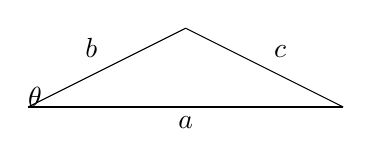
\begin{tikzpicture}
            \coordinate (C) at (0, 0);
            \coordinate (B) at (4, 0);
            \coordinate (A) at (2, 1);

            \draw (C) -- (B) node [midway,anchor=north] {$a$};
            \draw (B) -- (A) node [midway,anchor=south west] {$c$};
            \draw (A) -- (C) node [midway,anchor=south east] {$b$};

            \tkzMarkAngle[size=0.3cm,mark=|](C,A,B)
            \tkzLabelAngle[pos=0.6](C,A,B) {$\theta$}
        \end{tikzpicture}
    \caption{Law of Cosines}
    \label{fig:law-of-cosines}
    \end{figure}

    We can use this to extend our notion of angle beyond $\R^2$. Let $a = \norm{x - y}$, $b = \norm{x}$, and $c = \norm{y}$ as in Figure \ref{fig:vector-law-of-cosines}. Then $\norm{x - y}^2 = \langle x-y, x-y \rangle = \langle x, x\rangle - 2\langle x, y\rangle + \langle y, y \rangle = \norm{x}^2 - 2\langle x, y \rangle + \norm{y}^2$. Applying the Law of Cosines, we obtain
    \[\cos(\theta) = \frac{\langle x, y \rangle}{\norm{x}\norm{y}}.\]

    \begin{figure}[ht!]
        \centering
        \begin{tikzpicture}
            \coordinate (C) at (0, 0);
            \coordinate (B) at (4, 0);
            \coordinate (A) at (2, 1);

            \begin{scope}[decoration={
                markings,
                mark=at position 0.5 with {\arrow{>}}}
                ]
                \draw[postaction={decorate}] (A)--(B) node [midway,anchor=south west] {$y$};
                \draw[postaction={decorate}] (A)--(C) node [midway,anchor=south east] {$x$};
                \draw[postaction={decorate}] (B)--(C) node [midway,anchor=north] {$x-y$};
            \end{scope}
        \end{tikzpicture}
    \caption{Vector triangle}
    \label{fig:vector-law-of-cosines}
    \end{figure}
\end{rmk}

\begin{defn}
    Let $(V, \langle,\rangle)$ be an inner product space over $F$, and let $x, y \in V$ be non-zero vectors. We define the \emph{angle} between $x$ and $y$ as
    \[\theta = \arccos\left(\frac{\langle x, y \rangle}{\norm{x}\norm{y}}\right).\]
\end{defn}

\begin{defn}
    Let $(V, \langle,\rangle)$ be an inner product space over $F$. A subset $S \subseteq V$ is
    \begin{itemize}
        \item \emph{orthogonal} if $x$ and $y$ are orthogonal for every $x, y \in S$ where $x \neq y$,
        \item \emph{normal} if $\norm{x} = 1$ for all $x \in S$,
        \item \emph{orthonormal} if $S$ is both orthogonal and normal.
    \end{itemize}
\end{defn}

\begin{rmk}
    If $x \in V$ is non-zero, then $\frac{x}{\norm{x}}$ is a unit vector since
    \[\norm{\frac{x}{\norm{x}}} = \frac{1}{\norm{x}}\norm{x} = 1.\]
\end{rmk}

\begin{prop}
    Let $(V, \langle,\rangle)$ be an inner product space over $F$, and let $S \subseteq V$ be orthogonal. If all $x \in S$ are non-zero then $S$ is linearly independent.
\end{prop}

\begin{proof}
    Suppose that $a_1v_1 + \cdots + a_kv_k = \vec{0}$ for some distinct $v_1, \ldots, v_k \in S$ and non-zero $a_1, \ldots, a_k \in F$. Fix $j \in \{1, \ldots, k\}$. Then
    \begin{align*}
        0 &= \langle \vec{0}, v_j \rangle = \langle a_1v_1 + \cdots + a_kv_k, v_j \rangle \\
        &= a_1\langle v_1, v_j \rangle + \cdots + a_k\langle v_k, v_j \rangle.
    \end{align*}
    Since $S$ is orthogonal, all $\langle v_i, v_j \rangle$ must be zero except for $i = j$. Therefore, $0 = a_j\langle v_j, v_j \rangle$. Since $v_j \neq \vec{0}$, $\langle v_j, v_j \rangle \neq 0$ and therefore $a_j = 0$. It follows that all $a_1, \ldots, a_k = 0$ and so $S$ is linearly independent.
\end{proof}

\begin{exmp}
    \[S = \left\{(1, 1, 0), (1, -1, 1), (-1, 1, 2)\right\}\]
    $S$ can easily to verified to be orthogonal, and so it must be linearly independent and therefore forms a basis for $\R^3$. Furthermore, it follows that
    \[B = \left\langle \frac{1}{\sqrt{2}}(1, 1, 0), \frac{1}{\sqrt{3}}(1, -1, 1), \frac{1}{\sqrt{6}}(-1, 1, 2)\right\rangle\]
    is an orthonormal basis for $\R^3$.
\end{exmp}

\begin{thm}\label{orthogonal-decomposition}
    Let $(V, \langle,\rangle)$ be an inner product space over $F$, and let $S = \{v_1, \ldots, v_k\}$ be an orthogonal set of non-zero vectors. Given any $y \in \spanset{S}$, then $y$ is the sum of the orthogonal components of $y$ along each $v_i$:
    \[y = \sum_{i=1}^{k}\frac{\langle y, v_i\rangle}{\norm{v_i}^2}v_i.\]
\end{thm}

\begin{proof}
    Since $y \in \spanset{S}$, we know that $y = \sum_{i=1}^{k}a_iv_i$ for some $a_i \in F$. Fix $j \in \{1, \ldots, k\}$. Then
    \[\langle y, v_j \rangle = \left\langle \sum_{i=1}^{k}a_iv_i, v_j \right\rangle = a_j\langle v_j, v_j \rangle, \textrm{ and so } a_j = \frac{\langle y, v_j \rangle}{\langle v_j, v_j \rangle} = \frac{\langle y, v_j\rangle}{\norm{v_j}^2}.\]
\end{proof}

\begin{cor}\label{orthonormal-decomposition}
    If $S$ is orthonormal, then $y = \sum_{i=1}^{k}\langle y, v_i\rangle v_i$.
\end{cor}

\begin{thm}{Gram-Schmidt Process}\label{gram-schmidt-process}\proofbreak
    Let $(V, \langle,\rangle)$ be an inner product space over $F$, and let $S =\{w_1, \ldots, w_n\}$ be a linearly independent set. Define $S' = \{v_1, \ldots, v_n\}$ by $v_1 = w_1$, and for $k > 1$ by
    \[v_k = w_k - \sum_{i=1}^{k-1}\frac{\langle w_k, v_i\rangle}{\norm{v_i}^2}v_i.\]
    Then $S'$ is an orthogonal set of non-zero vectors, and has the same span as $S$.
\end{thm}

\begin{proof}
    Let $S_k = \{w_1, \ldots, w_k\}$ and $S_{k}' = \{v_1, \ldots, v_k\}$. We will show by induction on $k$ that $S_{k}'$ is an orthogonal set of non-zero vectors such that $\spanset{S_k} = \spanset{S_{k}'}$.

    When $k = 1$, $S_k = \{w_1\} = \{v_1\} = S_{k}'$ and so $S_{k}'$ is vacuously orthogonal, and $v_1 \neq \vec{0}$. Assume that the statement holds for some $k-1 \geq 1$. Then
    \begin{align*}
        v_k = w_k - \sum_{i=1}^{k-1}\frac{\langle w_k, v_i\rangle}{\norm{v_i}^2}v_i.
    \end{align*}
    Suppose that $v_k = \vec{0}$, then
    \[w_k = \sum_{i=1}^{k-1}\frac{\langle w_k, v_i\rangle}{\norm{v_i}^2}v_i,\]
    and so $w_k \in \spanset{S_{k-1}'} = \spanset{S_{k-1}}$. However, this violates the assumption that $S_{k-1}$ is linearly independent. Therefore, $v_k \neq \vec{0}$. For $j \in \{1, \ldots, k-1\}$,
    \begin{align*}
        \langle v_k, v_j \rangle = \langle w_k, v_j \rangle - \sum_{i=1}^{k-1}\frac{\langle w_k, v_i}{\norm{v_i}^2}\langle v_i, v_j \rangle = \langle w_k, v_j \rangle - \frac{\langle w_k, v_j}{\norm{v_j}^2}\langle v_j, v_j \rangle = 0,
    \end{align*}
    and so $S_{k}'$ must be orthogonal.

    By construction, $v_k \in \spanset{S_k}$, and so $\spanset{S_{k}'}$ is a subspace of $\spanset{S_{k}}$. Since $S_{k}$ and $S_{k}'$ are linearly independent and each have $k$ vectors, they must have the same dimension. Then by Theorem \ref{subspace-is-finite}, it follows that $\spanset{S_{k}'} = \spanset{S_k}$.
\end{proof}

\begin{cor}
    Let $(V, \langle,\rangle)$ be a finite dimensional inner product space over $F$. Then $V$ has an orthonormal basis.
\end{cor}

\begin{proof}
    Let $B$ be any basis for $V$. Apply the Gram-Schmidt process to obtain an orthogonal basis $B'$, and finally normalize each vector in $B'$ to obtain an orthonormal basis for $V$.
\end{proof}

\begin{exmp}
    Consider $\R^4$ with the standard dot product, and let
    \[S = \{(1, 0, 1, 0), (1, 1, 1, 1), (0, 1, 2, 1)\}.\]
    We start with $v_1 = w_1 = (1, 0, 1, 0)$, and then
    \[v_2 = w_2 - \frac{\langle w_2, v_1\rangle}{\norm{v_1}^2}v_1 = (1, 1, 1, 1) - \frac{2}{2}(1, 0, 1, 0) = (0, 1, 0, 1),\]
    \[v_3 = w_3 - \frac{\langle w_3, v_1 \rangle}{\norm{v_1}^2}v_1 - \frac{\langle w_3, v_2 \rangle}{\norm{v_2}^2}v_2 = (0, 1, 2, 1) - \frac{2}{2}(1, 0, 1, 0) - \frac{2}{2}(0, 1, 0, 1) = (-1, 0, 1, 0).\]
    Therefore, $\{(1, 0, 1, 0), (0, 1, 0, 1), (-1, 0, 1, 0)\}$ is an orthogonal set, and
    \[\left\{\frac{1}{\sqrt{2}}(1, 0, 1, 0), \frac{1}{\sqrt{2}}(0, 1, 0, 1), \frac{1}{\sqrt{2}}(-1, 0, 1, 0)\right\}\]
    is an orthonormal set.
\end{exmp}

\begin{defn}
    Let $(V, \langle,\rangle)$ be an inner product space over $F$, and $S \subseteq V$ an arbitrary non-empty set. The \emph{orthogonal complement} of $S$ is the set
    \[S^{\perp} = \left\{x \in V \compbar \langle x, y \rangle = 0 \,\forall y \in S \right\}.\]
\end{defn}

\begin{lemma}\label{orthogonal-complement-is-subspace}
    Let $(V, \langle,\rangle)$ be an inner product space over $F$, and $S \subseteq V$ an arbitrary non-empty set. Then $S^{\perp}$ is a vector subspace of $V$.
\end{lemma}

\begin{proof}
    Since $\langle \vec{0}, y \rangle = 0$ for all $y \in S$, we know that $\vec{0} \in S^{\perp}$. For any $x, z \in S^{\perp}$ and $r \in F$, and for all $y \in S$
    \[\langle x + rz, y \rangle = \langle x, y \rangle + r\langle z, y \rangle = 0 + r(0) = 0,\]
    so $x + rz \in S^{\perp}$. Therefore, $S^{\perp}$ by a subspace of $V$ by Proposition \ref{subspace-proof}.
\end{proof}

\begin{exmp}
    Let $V$ be a vector space with an arbitrary inner product. Then $\{\vec{0}\}^{\perp} = V$ and $V^{\perp} = \{\vec{0}\}$.
\end{exmp}

\begin{exmp}
    In $\R^3$ with the standard dot product, $\{e_3\}^{\perp} = \spanset{\{e_1, e_2\}}$.
\end{exmp}

\begin{lemma}\label{orthogonal-complement-of-orthogonal-complement}
    Let $(V, \langle,\rangle)$ be an inner product space over $F$, and $S \subseteq V$ an arbitrary non-empty set. Then $S \subseteq \left(S^{\perp}\right)^{\perp}$.
\end{lemma}

\begin{proof}
    Fix some $x \in S$. For any $y \in S^{\perp}$, we know that $\langle x, y \rangle = 0$ by definition. But $\langle y, x \rangle = \overline{\langle x, y \rangle} = \overline{0} = 0$, and so $x \in \left(S^{\perp}\right)^{\perp}$.
\end{proof}

\begin{thm}
    Let $(V, \langle,\rangle)$ be a finite dimensional inner product space over $F$ and $W \subseteq V$ a subspace.
    \begin{enumerate}
        \item $W \intersection W^{\perp} = \{\vec{0}\}$.
        \item Any $x \in V$ can be uniquely expressed as $x = w + u$ where $w \in W$ and $u \in W^{\perp}$.
        \item The dimension of $V$ is the sum of the dimensions of $W$ and $W^{\perp}$.
        \item $W = \left(W^{\perp}\right)^{\perp}$.
    \end{enumerate}
\end{thm}

\begin{proof}\proofbreak
    (1) Let $x \in W \intersection W^{\perp}$. By definition, $\langle x, x \rangle = 0$, so $x = \vec{0}$.

    Use the Gram-Schmidt process to construct an orthonormal basis $\{v_1, \ldots, v_n\}$ for $V$ such that $\{v_1, \ldots, v_k\}$ forms an orthonormal basis for $W$. We will show that $\{v_{k+1}, \ldots, v_n\}$ forms an orthonormal basis for $W^{\perp}$. First note that $\{v_{k+1}, \ldots, v_n\}$ is linearly independent by construction. Let $x \in V$, then by Corollary \ref{orthonormal-decomposition}
    \[x = \sum_{i=1}^{n}\langle x, v_i\rangle v_i.\] In the case that $x \in W^{\perp}$, by definition $\langle x, v_i\rangle = 0$ and so $x \in \spanset{\{v_{k+1}, v_n\}}$, and so $W^{\perp} \subseteq \spanset{\{v_{k+1}, \ldots, v_n\}}$. Furthermore, for $y \in \spanset{\{v_{k+1}, \ldots, v_n\}}$ we know that \[y = \sum_{i={k+1}}^{n}\langle x, v_i\rangle v_i = \sum_{i=1}^{n}\langle x, v_i\rangle v_i.\] Since $\{v_1, \ldots, v_k\}$ is linearly independent, it follows that $\langle y, v_i \rangle = 0$ and so $\langle y, w \rangle = 0$ for all $w \in \spanset{\{v_1, \ldots, v_k\}} = W$. Therefore, $y \in W^{\perp}$ and so $\spanset{\{v_{k+1}, \ldots, v_n\}} \subseteq W^{\perp}$, implying that $\spanset{\{v_{k+1}, \ldots, v_n\}} = W^{\perp}$. It follows that $\{v_{k+1}, v_n\}$ is a basis for $W^{\perp}$ by definition.

    (2) Let $x \in V$, then \[x = \sum_{i=1}^{n}\langle x, v_i \rangle v_i = \sum_{i=1}^{k}\langle x, v_i \rangle v_i = \sum_{i={k+1}}^{n}\langle x, v_i \rangle v_i = w + u,\] where $w \in W$ and $u \in W^{\perp}$. Therefore, there is at least one way to express $x \in V$ as $x = w + u$ where $w \in W$ and $u \in W^{\perp}$. To show uniqueness, assume that $x = w + u = w' + u'$ where $w, w' \in W$ and $u + u' \in W^{\perp}$. Then $w + u = w' + u'$, and so $w - w' = u - u' \in W \intersection W^{\perp} = \{\vec{0}\}$ by (1), and so $w = w'$ and $u = u'$.

    (3) Since $\{v_1, \ldots, v_k\}$ is a basis for $W$ and $\{v_{k+1}, \ldots, v_n\}$ is a basis for $W^{\perp}$, it necessarily follows that the dimension of $V$ is the sum of the dimensions of $W$ and $W^{\perp}$.

    (4) By (3), we know that $\dim V = \dim W + \dim W^{\perp}$ and also that $\dim V = \dim W^{\perp} + \dim\left(W^{\perp}\right)^{\perp}$, so $\dim W = \dim \left(W^{\perp}\right)^{\perp}$. Since $W$ and $\left(W^{\perp}\right)$ are both subspaces of $V$ by Lemma \ref{orthogonal-complement-is-subspace} and $W \subseteq \left(W^{\perp}\right)^{\perp}$ by Lemma \ref{orthogonal-complement-of-orthogonal-complement}, we know that $\dim W = \dim \left(W^{\perp}\right)^{\perp}$ implies that $W = \left(W^{\perp}\right)^{\perp}$ by Proposition \ref{subspace-is-finite}.
\end{proof}

\begin{defn}
    Let $V$ be a vector space over $F$, and $W$ and $U$ subspaces of $V$. If $W \intersection U = \{\vec{0}\}$, and every $x \in V$ can be uniquely expressed as $x = w + u$ with $w \in W$ and $u \in U$, we say that $V$ is the \emph{direct sum} of $W$ and $U$, denoted as $V = W \directsum U$.
\end{defn}

\begin{exmp}
    Let $(V, \langle,\rangle)$ be a finite dimensional inner product space over $F$ and $W \subseteq V$ a subspace. Then $V = W \directsum W^{\perp}$.
\end{exmp}

\begin{exmp}
    $\R^3 = \spanset{\{e_1, e_2\}} \directsum \spanset{\{e_3\}}$.
\end{exmp}

\begin{defn}
    Let $(V, \langle,\rangle)$ be a finite dimensional inner product space over $F$ and $W \subseteq V$ a subspace. For $x = w + u \in V$ where $w \in W$ and $u \in W^{\perp}$, we say that $w$ is the \emph{orthogonal projection} of $x$ onto $W$.
\end{defn}

\begin{rmk}
    If $\{v_1, \ldots, v_k\}$ is an orthonormal basis for $W$ and $x \in V$, then the orthogonal projection $w$ of $x$ on $W$ is
    \[w = \sum_{i=1}^{k}\langle x, v_i \rangle v_i, \;\textrm{and}\, u = x - w.\]
\end{rmk}

\begin{prop}\label{ortho-proj-closest}
    Let $(V, \langle,\rangle)$ be a finite dimensional inner product space over $F$ and $W \subseteq V$ a subspace. The orthogonal projection $w$ of $x$ is the unique vector in $W$ that is closest to $x$ --- that is, $\norm{x - w} \leq \norm{x - y}$ for all $y \in W$, with equality if and only if $y = w$.
\end{prop}

\begin{proof}
    Let $w$ be the orthogonal projection of $x$ on $W$, and $u = x - w \in W^{\perp}$. Since $w, y \in W$ we have $w - y \in W$, and so $w - y$ is orthogonal to $u$. Then $\norm{x-y}^2 = \norm{w + u - y}^2$ and by the Pythagorean Theorem \ref{pythagorean-thm} we have $\norm{w + u - y}^2 = \norm{w - y}^2 + \norm{u^2}$. It follows that
    \[\norm{x-y}^2 = \norm{w - y}^2 + \norm{u^2} \geq \norm{u^2} = \norm{x - w}^2.\]
\end{proof}

\section{Adjoints}

\begin{defn}
    Let $(V, \langle, \rangle_V)$ and $(W, \langle, \rangle_W)$ be inner product spaces over $F$. Given a linear transformation $T: V \to W$, the \emph{adjoint} of $T$ is the linear transformation $T^{*}: W \to V$ satisfying \[\langle T(V), W\rangle_W = \langle V, T^{*}(W)\rangle_V.\]
\end{defn}

\begin{lemma}Representation Theorem\label{adjoint-representation-theorem}\proofbreak
    Let $(V, \langle,\rangle)$ be a finite dimensional inner product space over $F$, and let $\ell: V \to F$. There exists unique $w \in V$ such that $\ell(v) = \langle v, w \rangle$ for all $v \in V$.
\end{lemma}

\begin{proof}
    Let $\{v_1, \ldots, v_n\}$ be an orthonormal basis for $V$. For any $v \in V$, we know that
    \[v = \sum_{i=1}^{n}\langle v, v_i \rangle v_i,\]
    and so it follows that
    \[\ell(v) = \ell\left(\sum_{i=1}^{n}\langle v, v_i \rangle v_i\right) = \sum_{i=1}^{n}\langle v, v_i \rangle \ell(v_i) = \left\langle v, \sum_{i=1}^{n}\overline{\ell(v_i)v_i} \right\rangle.\]
    Therefore, $w = \sum_{i=1}^{n}\overline{\ell(v_i)v_i}$. Uniqueness follows from Theorem \ref{inner-product-properties} (5).
\end{proof}

\begin{thm}\label{adjoint-existence-uniqueness}
    Let $(V, \langle, \rangle)$ and $(W, \langle, \rangle)$ be inner product spaces over $F$, and $T: V \to W$ be a linear transformation. The adjoint $T^*$ of $T$ exists and is unique.
\end{thm}

\begin{proof}
    For given $w \in W$, consider $\ell: V \to F$ defined by $v \mapsto \langle T(v), w \rangle$. Since $T$ is linear in $v$ and $\langle,\rangle$ is linear in the first argument, $\ell$ is linear in $v$. By Lemma \ref{adjoint-representation-theorem}, there exists unique $y \in V$ such that $\langle T(v), w \rangle = \ell(v) = \langle v, y \rangle$. Define $T^*(w) = y$ to obtain a function $T^*: W \to V$.

    All that remains is for us to show that $T^*$ is indeed a linear function. Note that
    \begin{align*}
        \langle v, T^*(w_1 + rw_2) \rangle &= \langle T(v), w_1 + rw_2 \rangle = \langle T(v), w_1 \rangle + \overline{r}\langle T(v), w_2 \rangle \\
        &= \langle v, T^*(w_1) \rangle + \overline{r}\langle v, T^*(w_2) \rangle = \langle v, T^*(w_1) + rT^*(w_2) \rangle.
    \end{align*}
    It follows that $T^*(w_1 + rw_2) = T^*(w_1) + rT^*(w_2)$ by Theorem \ref{inner-product-properties} (5). Therefore, $T^*$ is linear and is the unique function satisfying $\langle T(v), w \rangle = \langle v, T^*(w) \rangle$.
\end{proof}

\begin{prop}
    Let $(V, \langle, \rangle)$ and $(W, \langle, \rangle)$ be inner product spaces over $F$, and $T: V \to W$ be a linear transformation. Then
    \[(T^*)^* = T.\]
\end{prop}

\begin{proof}
    \[\langle T(v), w \rangle = \langle v, T^*(w) \rangle = \langle v, T^*(w) \rangle = \overline{\langle T^*(w), v \rangle} = \overline{\langle w, (T^*)^*(v) \rangle} = \langle (T^*)^*(v), w \rangle\]
\end{proof}

\begin{lemma}
    Let $A \in M_{m \times n}(F)$, $x \in F^n$, and $y \in F^m$. Then $\langle Ax, y \rangle_m = \langle x, A^{*}y \rangle_n$, where $\langle,\rangle_k$ denotes the standard dot product with in $F^k$.
\end{lemma}

\begin{proof}
    \[\langle x, A^{*}y\rangle_n = (A^{*}y)^{*}x = y^{*}(A^*)^{*}x = y^*Ax = \langle Ax, y \rangle_m\]
\end{proof}

\begin{rmk}
    Let $A$ be a matrix and $L_A$ the corresponding linear transformation. This lemma states that the linear transformation corresponding to the conjugate transpose of $A^{*}$ satisfies the adjoint property for the standard dot product, and so by Theorem \ref{adjoint-existence-uniqueness} is the unique adjoint. This is,
    \[\left(L_A\right)^{*} = L_{A^{*}}.\]
\end{rmk}

\begin{lemma}
    Let $A \in M_{m \times n}(F)$. Then the ranks of $A$ and $A*A$ are equal.
\end{lemma}

\begin{proof}
    Note that $A$ is $m \times n$, so $A^*A$ is an $n \times n$ square matrix. If we can show that the nullity of $L_A$ is equal to the nullity $L_{A^*A}$, then by the Rank-nullity Theorem \ref{rank-nullity} $A$ and $A^*A$ must have the same rank.

    For any $x$ in the kernel (null-space) of $L_A$, we have $Ax = \vec{0}$, and so $A^*Ax = A^*\vec{0} = \vec{0}$, and so the kernel of $L_A$ is a subset of the kernel of $L_{A^*A}$. Now consider $x$ in the kernel of $L_{A^*A}$. We know that
    \begin{align*}
        \langle Ax, Ax \rangle = \langle x, A^*Ax \rangle = \langle x, \vec{0} \rangle = 0,
    \end{align*}
    and so $Ax = \vec{0}$ by Theorem \ref{inner-product-properties} (4). Therefore, the kernel of $L_{A^*A}$ is also a subset of the kernel of $L_A$, and so the kernels (and therefore the nullities) of $L_A$ and $L_{A^*A}$ are equal.
\end{proof}

\begin{rmk}
    Note that since $A^*A$ is an $n \times n$ matrix, it is invertible precisely when the rank of $A$ is $n$.
\end{rmk}

\begin{thm}
    Let $A \in M_{m \times n}(F)$ and $y \in F^n$. Then there exists $x_0 \in F^n$ such that
    \[\norm{y - Ax_0} \leq \norm{y - Ax}.\]
    Furthermore, if $A$ has rank $n$, then $x_0$ is unique and is given by $x_0 = (A^*A)^{-1}A^*y$.
\end{thm}

\begin{proof}
    Let $W$ be the column space of $A$, and let $w_0$ be the orthogonal projection of $y$ onto $W$. We know that $w_0$ is the unique vector in the column space of $A$ that satisfies $\norm{y - w_0} \leq \norm{y - w}$ for all $w$ in the column space of by Proposition \ref{ortho-proj-closest}. Since $w_0$ is the in column space of $A$, we are guaranteed the existence (although not the uniqueness) of $x_0$, which is simply the coordinates of $w_0$ in terms of the columns of $A$. If $A$ has rank $n$ then the columns of $A$ form a basis for the column space and so $x_0$ must be unique.

    When $A$ has rank $n$, then $x_0$ satisfies $y = Ax_0 + u$ where $u \in W^{\perp}$ and $Ax \in W$. Therefore, $y - Ax_0 = u \in W^{\perp}$, so for all $x \in F^n$ we have
    \[\langle Ax, y - Ax_0 \rangle = 0,\]
    and so $\langle x, A^*y - A^*Ax_0 \rangle = 0$. Then since this equation is true for all $x \in F^n$ we must have $A^*y - A^*Ax_0 = \vec{0}$, and so $A^*Ax_0 = A^*y$. Since $A^*A$ is invertible when $A$ has rank $n$, we finally have
    \[x_0 = \left(A^*A\right)^{-1}A^*y.\]
\end{proof}

\begin{defn}
    A matrix $P \in M_{n \times n}(\C)$ is said to be \emph{orthogonal} when the columns of $P$ form an orthogonal basis for $\C^n$.
\end{defn}

\begin{lemma}
    A matrix $P \in M_{n \times n}(\C)$ is orthogonal if and only if $P$ is invertible and $P^{-1} = P^{\transpose}$.
\end{lemma}

\begin{proof}
    Let $v_i$ denote the $i$th column of $P$ (and therefore the $i$th column of $P^{\transpose}$). Note that $P$ is orthogonal is equivalent to saying that $v_i \cdot v_j = 1$ precisely when $i = j$ and $v_i \cdot v_j = 0$ otherwise. Therefore, $P$ is orthogonal is equivalent to $P^{\transpose}P = I_n$ and since $P^{\transpose}$ is also orthogonal, $PP^{\transpose} = I_n$. It follows that $P$ is orthogonal is precisely equivalent to $P$ is invertible and $P^{-1} = P^{\transpose}$.
\end{proof}

\begin{rmk}
    If $P$ is orthogonal, then so is $P^{\transpose}$. If $S$ and $R$ are orthogonal, then $SR$ is orthogonal since $(SR)(SR)^{\transpose} = S(RR^{\transpose})S^{\transpose} = SS^{\transpose} = I$.
\end{rmk}

\begin{thm}Spectral Theorem\label{spectral-theorem}\proofbreak
    Let $A \in M_{n \times n}(\R)$. If $A$ is symmetric ($A = A^{\transpose}$), then $A$ is diagonalizable and there exists an orthogonal basis for $\R^n$ composed of eigenvectors of $A$.
\end{thm}

\begin{proof}
    Consider $A \in M_{n \times n}(\C)$. We know that $A$ must have at least one eigenvalue $\lambda \in \C$ by the Fundamental theorem of algebra \ref{algebra-fundamental-theorem}.
    \begin{align*}
        \lambda\langle x, x\rangle = \langle Ax, x \rangle = \langle x, A^*x\rangle
    \end{align*}
    Since $A \in M_{n \times n}(\R)$, $A^* = A^{\transpose}$. Then $A = A^{\transpose}$ implies that $A^* = A$, so $\langle x, A^*x \rangle = \langle x, Ax \rangle$. We then have
    \begin{align*}
        \lambda\langle x, x\rangle = \langle x, \lambda x\rangle = \overline{\lambda}\langle x, x \rangle.
    \end{align*}
    Since $x \neq 0$, it follows that $\lambda = \overline{\lambda}$ and so $\lambda \in \R$. Therefore, all eigenvectors of $A$ are real and so $A$ has at least one real eigenvector.

    We will proceed by induction on $n$. First, a $1 \times 1$ matrix $A = (a)$ is trivially both symmetric and diagonalizable, and $\{(1)\}$ is a basis for $\R^1$ that is vacuously orthogonal and composed of eigenvectors of $A$. Now assume that for $m \leq n-1$, any $m \times m$ real symmetric matrix is diagonalizable, and there exists an orthogonal basis for $\R^m$ composed of its eigenvectors.
    
    Let $v_1$ be an eigenvector and $\lambda_1$ the corresponding eigenvalue. Complete to an ordered orthogonal basis $\langle v_1, \ldots, v_n \rangle$ for $\R^n$. Let $Q$ be a matrix whose $i$th column is $v_i$, and let
    $\tilde{A} = [L_A]_{B}^{B}$. Then $\tilde{A} = Q^{-1}AQ = Q^{\transpose}AQ$. Note that $\tilde{A}$ is symmetric: $\left(Q^{\transpose}AQ\right)^{\transpose} = Q^{\transpose}A^{\transpose}\left(Q^{\transpose}\right)^{\transpose} = Q^{\transpose}AQ = \tilde{A}$.

    Since $Av_1 = \lambda_1v_1$, we know that
    \[\tilde{A} = \left(\begin{array}{c|ccc}
        \lambda_1 & 0 & \cdots & 0 \\
        \hline
        0 & & & \\
        \vdots & & & \\
        0 & \largeblock{3}{2.2}{$B$}
    \end{array}\right),\]
    where $B$ is an $(n-1)\times(n-1)$ real symmetric matrix. By assumption, there exists an $(n-1)\times(n-1)$ diagonal matrix $E$ and $T$ an $(n-1)\times(n-1)$ orthogonal matrix such that $B = TET^{-1} = TET^{\transpose}$. Then
    \[\tilde{A} = \left(\begin{array}{c|ccc}
        1 & 0 & \cdots & 0 \\
        \hline
        0 & & & \\
        \vdots & & & \\
        0 & \largeblock{3}{2.0}{$T$}
    \end{array}\right)
    \left(\begin{array}{c|ccc}
        \lambda_1 & 0 & \cdots & 0 \\
        \hline
        0 & & & \\
        \vdots & & & \\
        0 & \largeblock{3}{2.0}{$E$}
    \end{array}\right)
    \left(\begin{array}{c|ccc}
        1 & 0 & \cdots & 0 \\
        \hline
        0 & & & \\
        \vdots & & & \\
        0 & \largeblock{3}{2.7}{$T^{\transpose}$}
    \end{array}\right) = SDS^{\transpose},\]
    where $S$, $D$, and $S^{\transpose}$ are simply the three matrices in the product. Then,
    \[A = Q\tilde{A}Q^{\transpose} = QSDS^{\transpose}Q^{\transpose} = (QS)D(QS)^{\transpose} = (QS)D(QS)^{-1}.\]
    Note that $D$ is diagonal since $E$ is, and $S$ (and $S^{\transpose}$) are orthogonal since $T$ (and $T^{\transpose})$) is. Since $Q$ and $S$ are orthogonal, so is their product $QS$. Since $D$ is a diagonal matrix of eigenvalues, the columns of $QS$ are necessarily eigenvectors of $A$, and so the columns of $QS$ form an orthogonal basis of eigenvectors.
\end{proof}
